
\documentclass[conference]{IEEEtran}

% *** CITATION PACKAGES ***
%
% cite.sty was written by Donald Arseneau
% V1.6 and later of IEEEtran pre-defines the format of the cite.sty package
% \cite{} output to follow that of the IEEE. Loading the cite package will
% result in citation numbers being automatically sorted and properly
% "compressed/ranged". e.g., [1], [9], [2], [7], [5], [6] without using
% cite.sty will become [1], [2], [5]--[7], [9] using cite.sty. cite.sty's
% \cite will automatically add leading space, if needed. Use cite.sty's
% noadjust option (cite.sty V3.8 and later) if you want to turn this off
% such as if a citation ever needs to be enclosed in parenthesis.
% cite.sty is already installed on most LaTeX systems. Be sure and use
% version 5.0 (2009-03-20) and later if using hyperref.sty.
% The latest version can be obtained at:
% http://www.ctan.org/pkg/cite
% The documentation is contained in the cite.sty file itself.
%
%
%% *** GRAPHICS RELATED PACKAGES ***
%% 
%\usepackage[pdftex]{graphicx}

% *** MATH PACKAGES ***
%

% A popular package from the American Mathematical Society that provides
% many useful and powerful commands for dealing with mathematics.
%
% Note that the amsmath package sets \interdisplaylinepenalty to 10000
% thus preventing page breaks from occurring within multiline equations. Use:
% after loading amsmath to restore such page breaks as IEEEtran.cls normally
% does. amsmath.sty is already installed on most LaTeX systems. The latest
% version and documentation can be obtained at:
% http://www.ctan.org/pkg/amsmath

% *** SPECIALIZED LIST PACKAGES ***
%
% algorithmic.sty was written by Peter Williams and Rogerio Brito.
% This package provides an algorithmic environment fo describing algorithms.
% You can use the algorithmic environment in-text or within a figure
% environment to provide for a floating algorithm. Do NOT use the algorithm
% floating environment provided by algorithm.sty (by the same authors) or
% algorithm2e.sty (by Christophe Fiorio) as the IEEE does not use dedicated
% algorithm float types and packages that provide these will not provide
% correct IEEE style captions. The latest version and documentation of
% algorithmic.sty can be obtained at:
% http://www.ctan.org/pkg/algorithms
% Also of interest may be the (relatively newer and more customizable)
% algorithmicx.sty package by Szasz Janos:
% http://www.ctan.org/pkg/algorithmicx


% *** ALIGNMENT PACKAGES ***
%
%\usepackage{array}
% Frank Mittelbach's and David Carlisle's array.sty patches and improves
% the standard LaTeX2e array and tabular environments to provide better
% appearance and additional user controls. As the default LaTeX2e table
% generation code is lacking to the point of almost being broken with
% respect to the quality of the end results, all users are strongly
% advised to use an enhanced (at the very least that provided by array.sty)
% set of table tools. array.sty is already installed on most systems. The
% latest version and documentation can be obtained at:
% http://www.ctan.org/pkg/array



% IEEEtran contains the IEEEeqnarray family of commands that can be used to
% generate multiline equations as well as matrices, tables, etc., of high
% quality.



% *** SUBFIGURE PACKAGES ***
%\ifCLASSOPTIONcompsoc
%  \usepackage[caption=false,font=normalsize,labelfont=sf,textfont=sf]{subfig}
%\else
%  \usepackage[caption=false,font=footnotesize]{subfig}
%\fi
% subfig.sty, written by Steven Douglas Cochran, is the modern replacement
% for subfigure.sty, the latter of which is no longer maintained and is
% incompatible with some LaTeX packages including fixltx2e. However,
% subfig.sty requires and automatically loads Axel Sommerfeldt's caption.sty
% which will override IEEEtran.cls' handling of captions and this will result
% in non-IEEE style figure/table captions. To prevent this problem, be sure
% and invoke subfig.sty's "caption=false" package option (available since
% subfig.sty version 1.3, 2005/06/28) as this is will preserve IEEEtran.cls
% handling of captions.
% Note that the Computer Society format requires a larger sans serif font
% than the serif footnote size font used in traditional IEEE formatting
% and thus the need to invoke different subfig.sty package options depending
% on whether compsoc mode has been enabled.
%
% The latest version and documentation of subfig.sty can be obtained at:
% http://www.ctan.org/pkg/subfig


% *** FLOAT PACKAGES ***
%
%\usepackage{fixltx2e}
% fixltx2e, the successor to the earlier fix2col.sty, was written by
% Frank Mittelbach and David Carlisle. This package corrects a few problems
% in the LaTeX2e kernel, the most notable of which is that in current
% LaTeX2e releases, the ordering of single and double column floats is not
% guaranteed to be preserved. Thus, an unpatched LaTeX2e can allow a
% single column figure to be placed prior to an earlier double column
% figure.
% Be aware that LaTeX2e kernels dated 2015 and later have fixltx2e.sty's
% corrections already built into the system in which case a warning will
% be issued if an attempt is made to load fixltx2e.sty as it is no longer
% needed.
% The latest version and documentation can be found at:
% http://www.ctan.org/pkg/fixltx2e


%\usepackage{stfloats}
% stfloats.sty was written by Sigitas Tolusis. This package gives LaTeX2e
% the ability to do double column floats at the bottom of the page as well
% as the top. (e.g., "\begin{figure*}[!b]" is not normally possible in
% LaTeX2e). It also provides a command:
%\fnbelowfloat
% to enable the placement of footnotes below bottom floats (the standard
% LaTeX2e kernel puts them above bottom floats). This is an invasive package
% which rewrites many portions of the LaTeX2e float routines. It may not work
% with other packages that modify the LaTeX2e float routines. The latest
% version and documentation can be obtained at:
% http://www.ctan.org/pkg/stfloats
% Do not use the stfloats baselinefloat ability as the IEEE does not allow
% \baselineskip to stretch. Authors submitting work to the IEEE should note
% that the IEEE rarely uses double column equations and that authors should try
% to avoid such use. Do not be tempted to use the cuted.sty or midfloat.sty
% packages (also by Sigitas Tolusis) as the IEEE does not format its papers in
% such ways.
% Do not attempt to use stfloats with fixltx2e as they are incompatible.
% Instead, use Morten Hogholm'a dblfloatfix which combines the features
% of both fixltx2e and stfloats:
%
% \usepackage{dblfloatfix}
% The latest version can be found at:
% http://www.ctan.org/pkg/dblfloatfix


% *** PDF, URL AND HYPERLINK PACKAGES ***
%\usepackage{url}
% url.sty was written by Donald Arseneau. It provides better support for
% handling and breaking URLs. url.sty is already installed on most LaTeX
% systems. The latest version and documentation can be obtained at:
% http://www.ctan.org/pkg/url
% Basically, \url{my_url_here}.


% *** Do not adjust lengths that control margins, column widths, etc. ***
% *** Do not use packages that alter fonts (such as pslatex).         ***
% There should be no need to do such things with IEEEtran.cls V1.6 and later.
% (Unless specifically asked to do so by the journal or conference you plan
% to submit to, of course. )

\usepackage{cite}
\usepackage{amsmath}
\interdisplaylinepenalty=2500
\usepackage[vlined,linesnumbered,algoruled]{algorithm2e}
\usepackage{multirow}
\usepackage{graphicx}

% correct bad hyphenation here
\hyphenation{op-tical net-works semi-conduc-tor}

\usepackage{csquotes}

\usepackage{array}
\newcolumntype{C}[1]{>{\centering\let\newline\\\arraybackslash\hspace{0pt}}m{#1}}

\begin{document}

\title{The State of Monte Carlo Neutron Transport: \\
The Role of GPUs and Portable Performance Abstractions }

\author{\IEEEauthorblockN{Ryan Bleile}
\IEEEauthorblockA{School of Computer and Information Science\\
University of Oregon\\
Eugene, Oregon 97403\\
Email: rbleile@cs.uoregon.edu}
}

% make the title area
\maketitle

% As a general rule, do not put math, special symbols or citations
% in the abstract
\begin{abstract}
Since near the beginning of electronic computing, Monte Carlo neutron transport has been a fundamental approach to solving nuclear physics problems.
%
Over the past few decades Monte Carlo transport applications have seen a significant increase in their capabilities and a reduction in time to solution.
%
Research efforts have been focused on areas such as scalability with distributed memory parallelism, load balance with domain decomposition, and variance reduction techniques.
%
In the last few years, however, the landscape has been changing.
%
Due to the high computational demands and inherently parallel nature of these applications, Monte Carlo transport applications are often used in the supercomputing environment.
%
Supercomputers are changing, in that they are becoming increasingly more parallel on a node, with GPGPUs and/or Xeon Phi co-processors powering the bulk of the compute capabilities.
%
In order to fully utilize the new machines' capabilities, it is becoming ever more important to migrate to a many-core perspective of any computing algorithm.
%
Monte Carlo transport applications, like many others, have the potentially difficult task of figuring out how to effectively utilize this new hardware.
%
Many groups have taken the initial steps to look into this problem or have focused their efforts on a sub-problem, such as continuous energy lookups.
%
In other fields, portable performance abstractions are presented as a promising approach to achieve parallelism and portability.
%
These abstractions provide the foundations for applications to write code once and run on any supported platform.
%
This paper describes the state of the art in Monte Carlo neutron transport, with a special emphasis on upcoming architectures.
%
\end{abstract}

\newpage

\tableofcontents

\newpage

% no keywords

% For peer review papers, you can put extra information on the cover
% page as needed:
% \ifCLASSOPTIONpeerreview
% \begin{center} \bfseries EDICS Category: 3-BBND \end{center}
% \fi
%
% For peerreview papers, this IEEEtran command inserts a page break and
% creates the second title. It will be ignored for other modes.
\IEEEpeerreviewmaketitle

%% Introduction Section %%
\section{ \textbf{Introduction}}

Today's supercomputer landscape is in flux.
%
Supercomputer architectures are undergoing more extreme changes than they have ever undergone in the past 20 years.
%
One big driving factor for this change are the concerns about power usage as we scale to larger and larger machines.
%
Modern machines are pushing up against a hard power limit meaning that in order to increase performance they must become more power efficient.
%
Traditionally, FLOPS/Watt is used to describe the relationship between power and performance.
%
Architectures are transitioning from fast and complex multi-core CPUs to much larger numbers of slower and simpler processors.
%
The amount of parallelism available on any given node in a supercomputer is growing by factors of hundreds or thousands because of this change.
%
This transition to many-core computing brings new and interesting challenges that need to be overcome.
%

%
In addition to the increase in node-level parallelism, it is unclear which many-core architecture choice will prove to be a winning design.
%
There are many different architectures to choose from when designing a supercomputer, and there is no obviously choice.
%
NVIDIA provides General Purpose Graphics Processing Units (GPGPUs) which are highly parallel throughput-optimized devices.
%
Intel provides Many Integrated Core (MIC) co-processors which provide large vector lanes and many threads.
%
Another option is Field Programmable Gate Arrays (FPGAs) which provide programmable logic circuits.
%
Across the Department of Energy (DOE) National Labs both the NVIDIA and Intel technologies are being pursued in their newest procurements ~\cite{coralWeb, trinityWeb}.
%

Application developers now face a complex and unclear path forward.
%
There are additional levels of complexity and potentially large application changes in order to effectively utilize this increase in parallelism.
%
In addition, an application developer cannot simply port to a new hardware architecture.
%
Instead, the application developer must address the issue of portability as well as performance of the algorithm or risk becoming outdated or unusable very quickly.
%
This problem is especially challenging when optimizations are architecture specific
%

%
Currently, there are a large number of physics and multi-physics applications that must understand how to navigate this complex and challenging landscape.
%
Simply porting to new architectures does not guarantee performance, and will still require applications to be ported individually to multiple architectures.
%
This paper will explore today's current efforts for portable performance solutions in the scope of one physics application, Monte Carlo particle transport.
%

%%%%%%%%%%%%%%%%%%%%%%%%%%%%%%%%%%%%%%%%%%%%%%%%%%%%%%%%%%%%%%%%%%%%%%%%%%%%%%%%%%%%%%

\section{ \textbf{What is Monte Carlo Particle Transport?}}

\begin{displayquote}
"The first thoughts and attempts I made to practice [the Monte Carlo method] were suggested by a question which occurred to me in 1946 as I was convalescing from an illness and playing solitaire. The question was what are the chances that a Canfield solitaire laid out with 52 cards will come out successfully? After spending a lot of time trying to estimate them by pure combinatorial calculations, I wondered whether a more practical method than "abstract thinking" might not be to lay it out say one hundred times and simply observe and count the number of successful plays. This was already possible to envisage with the beginning of the new era of fast computers, and I immediately thought of problems of neutron diffusion and other questions of mathematical physics, and more generally how to change processes described by certain differential equations into an equivalent form interpretable as a succession of random operations. Later... [in 1946, I ] described the idea to John von Neumann and we began to plan actual calculations."
\end{displayquote}
\begin{displayquote}
- Stan Ulam 1983 ~\cite{theMCM}
\end{displayquote}

John von Neumann became interested in Stan Ulam's idea and outlined how to solve the neutron diffusion and multiplication problems in fission devices.
%
Since this time Monte Carlo methods have continued to be a primary way for solving many questions in neutron transport~\cite{theMCM}.
%

\subsection{ \textbf{ Definition} }

In Computational Methods of Neuron Transport~\cite{LewisCMNT}, Lexis and Miller describe Monte Carlo transport as a simulation of some number of particle histories by using a random number generator.
%
For each particle history that is calculated, random numbers are generated and used to sample probability distributions describing the different physical events a particle can undergo, such as scattering angles or the length between collisions.
%
Ivan Lux and Laslo Koblinger further the previous definition in their book Monte Carlo Particle Transport Methods: Neutron and Photon Calculations:
%
\begin{displayquote}
"In all applications of the Monte Carlo method a stochastic model is constructed in which the expected value of a certain random variable (or of a combination of several variables) is equivalent to the value of a physical quantity to be determined. This expectation value is then estimated by the averaging of several independent samples representing the random variable introduced above. For the construction of the series of independent samples, random numbers following the distributions of the variable to be estimated are used." ~\cite{LuxMCPTM}
\end{displayquote}

% 
Estimating a quantity takes on the following mathematical form:
$$ \hat{x} = \frac{1}{N} \sum_{n=1}^{N} x_{n}, $$
where $x_{n}$ represents the contribution of the $n$th history for that quantity.
%
For the Monte Carlo method, we tally the $x_{n}$ from each particle history in order to compute the expected value $\hat{x}$~\cite{LewisCMNT}.
%

%
One very important question is how the estimated value $\hat{x}$ compares to the true value $\bar{x}$.
%
It turns out that the uncertainty in $\hat{x}$ decreases with increasing numbers of particle histories, and generally falls off asymptotically proportionate to $N^{-1/2}$~\cite{LewisCMNT}.
%

\subsection{ \textbf{ The Equation} }

%
The equation being solved by the neutron transport problem, shown below, displays each of the pieces that makes up a full Monte Carlo transport algorithm.
%
Large numbers of particles are used to create accurate estimations for each measured quantity.
%
The following equation is known as the Linearized Boltzmann transport equation for neutrons:
%
$$
\frac{1}{\nu} \frac{ \partial \Psi ( \vec{r}, E, \Omega, t ) }{\partial t}\ +\ 
(\nabla \cdot \Omega ) \Psi ( \vec{r}, E, \Omega, t )\ +\
$$
$$ 
\Sigma_a (\vec{r}, E ) \Psi ( \vec{r}, E, \Omega, t ) =$$
$$
\int _{E '} \int _{\Omega '} \Sigma_{s} ( \vec{r}, E', \Omega ' \rightarrow E, \Omega ) \Psi (\vec{r}, E, \Omega, t) d \Omega ' dE'\ +\ 
$$
$$
\chi (E) \int _{E'} \nu (E') \Sigma_{f} (\vec{r},E') \int _{\Omega '} \Psi ( \vec{r}, E, \Omega, t ) d \Omega ' dE'\ +\ $$
$$
S_ext(\vec{r}, E, \Omega, t )
$$
%
where $ \Psi ( \vec{r}, E, \Omega, t ) $ is angular flux, 
$\Sigma_a (\vec{r}, E )$ is the macroscopic cross section for particle absorption, 
$\Sigma_{s} ( \vec{r}, E', \Omega ' \rightarrow E, \Omega )$ is the macroscopic cross section for particle scattering,
$\Sigma_{f} (\vec{r},E') $ is the macroscopic cross section for particle production from a fission collision source,
$\chi (E)$ is a secondary particle spectrum from he fission process,
$\nu (E)$ is the average number of particles emitted per fission,
$S_ext(\vec{r}, E, \Omega, t )$ represents an external source,
$\vec{r}$ is the spacial coordinates,
$E$ is the energy,
$\Omega$ is angular direction,
and $t$ is the term for time~\cite{gentileMCPTAPO}.
%

\subsection{ \textbf{ Algorithm Approach} }

There are many ways to solve this problem.
%
The most common method is to track individual particle histories until a predetermined amount of particles has been simulated.
%
This method is known as the history-based approach.
%
In order to simulate a particle, the distance the particle must travel before it has any interactions must be computed and compared with all possible interactions.
%
The interaction with the shortest distance is chosen, followed by updating the particle and tallies based on the distance traveled and interaction occurring.
% 
Algorithm~\ref{alg:historybased} shows the history-based approach for a simple research code~\cite{alpsmc1} that has simple properties we can use to describe the method.
%
Algorithm~\ref{alg:mcmethod} shows the outer most scope of a Monte Carlo Problem for referencing where different optimizations or stages occur.
%
For example, Algorithm~\ref{alg:historybased} takes place inside the Cycle loop of Algorithm~\ref{alg:mcmethod} and shows only the steps for Cycle: Tracking.

\begin{algorithm}
\DontPrintSemicolon
\caption{History-based Monte Carlo algorithm}
\label{alg:historybased}
\ForEach{particle history}
{ 
    \While{particle not escaped or absorbed}
    {
       sample distance to collision in material\;
       sample distance to material interface\;
       compute distance to cell boundary\;
       select minimum distance, move particle, and perform event\;
       \If{particle escaped spatial domain}
       {
          update leakage tally\;
          end particle history\;
       }
       \If{particle absorbed}
       {
          update absorption tally\;
          end particle history\;
       }
    }
}
\end{algorithm}

\begin{algorithm}
\DontPrintSemicolon
\caption{Monte Carlo Method}
\label{alg:mcmethod}
Parse Inputs\;
\ForEach{Cycle}
{
	Initialize\;
	Tracking: Algorithm~\ref{alg:historybased}\;
	Finalize\;
}
Gather Tallies\;
\end{algorithm}






\section{ \textbf{ State of the Art Research} }

In order to understand the state of the art research in Monte Carlo transport, it is important to have some perspective on what has been done in the field already.
%
There is a long history of research and improvements for Monte Carlo transport problems and understanding this path, and the machines that the research was designed for, can help guide analysis of more recent efforts.
%
In the field of Monte Carlo transport, most research in the last 5 years has been related to GPGPU computing or has been physics based as opposed to computer science based research.
%
We will review and discuss the GPU research later in Section~\ref{sec:SOTAGPU}.
%
In this section we will look at the significant areas of interest when dealing with Monte Carlo transport applications that do not pertain to GPUs, namely Parallel performance on different architectures pre GPU computing, load balancing, optimizations in nuclear data look-ups, and variance reduction research.
%

	\subsection{ \textbf{ Parallel Performance }}

Since the inception of Monte Carlo particle transport over sixty years ago,
there has been tremendous growth as Monte Carlo applications have adapted to maximize performance on each architecture that has evolved over time.
%
The first models developed in 1947 would take five hours to compute 100 collisions, a task that today can be done in milliseconds.
%
In the 1940's and 1950's, Monte Carlo codes were written in very low level languages on the earliest computers.
%
The 1960's to 1980's saw a great increase in the capabilities of the Monte Carlo codes as computing power increased and codes become more fully featured.
%
In the 1980's Monte Carlo codes adopted parallel/vector machines.
%
In the 1990's Monte Carlo codes become more commonplace and parallelism increased to 100s or 1000s or processors through message passing with Parallel Virutal Machines (PVM)~\cite{pvm2011} or the Message Passing Interface (MPI)~\cite{blaiseMPI}.
%
In the 2000's multicore processors meant threading became more commonplace, mixing local and global forms of parallelism reaching tens of thousands of processors~\cite{brown2011recent}.
%

This growth in computer processing can also be categorized in terms of the styles of memory accesses.
%
Early systems were shared-memory environments almost exclusively.
%
Then distributed-memory systems became popular.
%
Finally, hybrid parallel systems, meaning systems that use both distributed- and shared-memory parallelism, became popular.
%
The following discussion is organized around these three types of parallelism.

\subsection*{ \textbf{Shared-Memory Performance}} 

Shared-memory systems refer to machines or models where all processors can access the same memory space.
%
Taking this a step further, in the unified memory architecture (UMA), all processors have access to the same memory and access to all memory takes the same amount of time~\cite{el2005advanced}.
%
One type of shared-memory system that was popular was the vector machine.
%
Vector machines took the shared-memory system and added additional synchronicity to the system by making all of the processors issue the same instruction~\cite{russell1978cray}.
%

\subsection*{Vector Machine Performance}

%
In the 1980's Monte Carlo transport algorithms began adapting ``event-based" methods.
%
The traditional history-based approach was not well suited for vector architectures, since the particle histories follow independent code paths.
%
In order to vectorize the algorithms and make them usable on the vector machine architectures, the codes had to be reorganized to follow the same code paths across independently computed particle histories.
%
By changing the algorithm to follow events instead of histories, the Monte Carlo method could be used in a vector based approach~\cite{martin1986monte}.
%

%
A common element for work in this area is that the vector approach is often related to a stack data structure.
%
The challenge then becomes properly organizing particles into the right sub-stack so that calculations can be performed~\cite{brown1984monte, bobrowicz1984vectorized}.
%
Another approach is to try to use only one main particle stack and pull off only the minimum information needed to compute each of the events into sub-stacks~\cite{martin1986monte}.
%
With each of these approaches particle events determine not only how the particles are organized but also what information is needed for processing. 
%
The main drawback to the event based approach is the added time for data movement or sorting.
%

%
Brown reported the potential for speedups of 20X-85X in his theoretical analysis of the use of event-based methods, and deemed this approach well worth the efforts required to change codes around in order to use this approach on vector machines ~\cite{brown1984monte}.
%
Martin's single big stack, sub-stack approach saw speedups randing from 5X to 12X depending on the problem choice and the machine he was running on~\cite{martin1986monte}.
%
Vujic and Martin vectorized and parallelized a reactor assembly code using explicit stacks and vectorizable data structures, reducing wall-clock time by 22X~\cite{vujic1991vectorization}.
%
Bobrowicz's explicit stack approach reached speedups of around 8X - 10X compared with the original history-based approach~\cite{bobrowicz1984vectorized}.
%
Finally, Burns used GAMTEB, the LANL Benchmark code, to show he could achieve similar performance to Bobrowicz by following a similar approach as Brown~\cite{burns1989vectorization}.
%

\subsection*{Multi-Threaded Architecture Performance}

%
Other shared-memory systems, separate from vector machines, were tried in this era.
%
One such machine was the Tera Multi-Threaded Architecture (MTA).
%
This approach focused on the use of parallel processors, hardware threading, and a shared-memory no cache design.
%
The idea was by focusing on threading they could mask away memory latency~\cite{majumdar2000parallel, snavely1998multi}.
%

%
Majumdar tried two methods of parallelizing the photon transport application TPHOT on the Tera MTA~\cite{majumdar2000parallel}. 
%
In TPHOT, looping occurred over spatial zones and energies of a region, with photons being computed when their containing region was processed. 
%
So for this application Majumdar chose to parallelize both over zones and over a combination of zones and energies through loop unrolling.
%
Table~\ref{tab:MTAPerf} shows that the parallelization on the MTA over zones and energies maintains incredible efficiency giving their application good speedups, while parallelizing over only zones does not expose enough parallel work to hide memory latency and so efficiency drops off quickly~\cite{majumdar2000parallel}.
%
\begin{table}
\caption {Parallel performance on the MTA using multithreaing~\cite{majumdar2000parallel}} \label{tab:MTAPerf} 
\begin{center}
\begin{tabular}{|c|c|c|c|}
\hline
Procs & Time (sec) & Speedup & Efficiency \\
\hline
\multicolumn{4}{|c|}{Parallelization by zones only} \\
\hline
1 & 764 & 1.00 & 1.00 \\
\hline
2 & 400 & 1.91 & 0.95 \\
\hline
4 & 227 & 3.37 & 0.84 \\
\hline
8 & 167 & 4.58 & 0.57 \\
\hline
\multicolumn{4}{|c|}{Parallelization by zones and energies} \\
\hline
1 & 745 & 1.00 & 1.00 \\
\hline
2 & 370 & 2.01 & 1.01 \\
\hline
4 & 187 & 3.98 & 0.99 \\
\hline
8 & 94 & 7.92 & 0.99 \\
\hline
\end{tabular}
\end{center}
\end{table}

More modern systems utilize shared-memory ideas as well, with a majority of the scientific efforts utilizing OpenMP threading models for shared-memory processing.
%
Often this model is overlooked in preference of distributed computing via MPI but that is not always the case.
%
Given an all particle method, OpenMP codes tend to scale with good efficiency with the only drawbacks having to do with possible atomic operations occuring the collection of output tallies.
%
In the case of no atomic operations and plenty of work, shared-memory implementations have nearly perfect efficiency on a node~\cite{siegel2014multi}.

\subsection*{ \textbf{Distributed-Memory Performance}}

One of the major transitions in supercomputing history came with the shift from vector computing to distributed-memory computing.
%
This type of computing is most often done with MPI and has, for the last 20 years, been a primary method of achieving parallel performance on small scale compute clusters and large scale supercomputers alike.
%
In the message passing model of parallelism, independent processes work together through the use of messages to synchronize actions or pass data between processors.
%
In this model, parallel efficiency is generally improved by spending more time working independently and is negatively affected by time spent sending messages or idled at a synchronization point~\cite{yanghybrid}.
%

%
The Monte Carlo particle transport history-based approach lends itself to the distributed model very well.
%
Each particle history is independent of any other particle histories and can be easily split up over processors~\cite{yanghybrid}.
%
However, moving to distributed memory systems creates complications in handling large and complex geometries.
%
Domain decomposition is typically used in this case, although it increases the complexity in using message passing.
%
Domain decomposition challenges are discussed further in Section 3.B.
%

%
Given the embarrassingly parallel nature of the Monte Carlo transport problem, the performance of this model produces results as expected.
%
As MPI processes increase, Monte Carlo transport continues to get a nearly linear speedup.
%
Majumdar shows that with 16 nodes and 8 MPI tasks per node, his biggest run, he was still able to achieve a 88\% efficiency~\cite{majumdar2000parallel} in his code that was parallel over zones and energies.
%
In an all particle code, Mercury at LLNL, parallel efficiencies of 80-90\% are seen when using MPI parallelism~\cite{procassini2005load}.

\subsection*{ \textbf{Distributed- + Shared-Memory Performance}}

%
Given the heterogenous nature of today's computing environment, and even in the fairly homogenous environment that has been prevalent, it is a common next step to consider combining distributed and shared-memory parallel schemes.
%
Shared-memory parallelism exists on a node or on one of the new accelerator devices.
%
Distributed-memory parallelism provides the opportunity for scaling to large supercomputers or clusters, giving users many nodes to work with.
%
Given the nature of these two models it is surprising how rarely they are combined.
%
Developers may have avoided using both types of parallelism to date since 
distributed-memory approaches work ``well enough" within a node, meaning
that each code on a node can be its own MPI task.
%
With the addition of accelerator architectures developers will no longer be able to ignore combining shared-memory and distributed-memory models
%

%
The combined distributed-shared model is often referred to as MPI+X~\cite{michaelwolfe2014}.
%
The X in this description being replaced with whichever shared-memory system is preferred.
%
The most common implementation of MPI+X to date is the MPI + OpenMP model.
%
In the MPI + OpenMP model, MPI is utilized for node to node communication and OpenMP is used for on node parallelism~\cite{michaelwolfe2014}.
%

%
Yang has recently shown that the MPI+OpenMP model has the benefit of achieving nearly perfect parallel efficiency and of significantly decreasing the memory overhead to an equivalent MPI only implementation.
%
He was able to show 82-84\% parallel efficiency and a decrease in memory cost from \textasciitilde1.4GB to \textasciitilde200MB for 8 processors~\cite{yanghybrid}.
%
Majumdar shows that with 16 nodes and 8 OpenMP threads per node, he was able to achieve a 95\% parallel efficiency which is an improvement over his MPI only method's 88\% parallel efficiency~\cite{majumdar2000parallel}. 
%

	\subsection{ \textbf{ Load Balance and Domain Decomposition} }

In order to achieve high levels of parallelism in transport problems with many geometries or zones, different parallel execution models are used.
%
Two primary models used are domain decomposition and replication.
%
Domain decomposition involves spatial decomposition of the geometry into domains, and then the assigning of processors to work on specific domains.
%
Replication involves storing the geometry information redundantly on each processor and assigning each processor a different set of particles.
~\cite{procassini2005load}
~\cite{o2005dynamic}


Load balance is often discussed in conjunction with domain decomposition since particles often migrate between different regions of a problem, meaning not all spatial domains will require the same amount of computational work.
%
In many applications there is at least one portion of the calculation that must be completed by all processors before all the processors can move forward with the calculation.
%
If one processor has more work than any other, all of the others must wait for that processor to complete its work~\cite{procassini2005load}~\cite{o2005dynamic}.
%
This load-imbalance can cause significant issues with scalability as parallelism is increased from hundreds to millions of processors ~\cite{o2013scalable}.
%

\subsection*{When to Load balance}

%
One key consideration when wanting to perform a load balance calculation, is to understand the cost of performing that calculation.
%
If too much time is spent making sure the problem is always perfectly load balanced, then computational resources are being wasted on a non-essential calculation, resulting is overall slower performance.
%
However, if too little resources are devoted to load-balancing than the problem will suffer from load-imbalance and the negative effects that entails.
%
One solution is to perform load balance at the start of each cycle or iteration of a Monte Carlo transport calculation, but only when that load balance will result in a faster overall calculation~\cite{o2005dynamic}.
%

An algorithm to determine when to load balance was explained in references~\cite{procassini2005load}~\cite{o2005dynamic}, where the following criterion could be checked inexpensively each cycle to determine if a load-balance operation should take place.
%
First, is to compute a speedup factor by comparing current parallel efficiency ($ \varepsilon_C $) to what parallel efficiency would be if processors were to redistribute their load ($ \varepsilon_{LB} $).
%
Second, is to predict the run time by using the time to execute the previous cycle($ \tau_{Phys} $), the speedup factor($S$), and finally, the time to compute the load balance itself($ \tau_{LB} $).
%
Finally, is to compare the predicted run with and without load balancing to determine if the operation is worthwhile.~\cite{o2005dynamic}


\begin{eqnarray}
S = \frac{\varepsilon_C}{\varepsilon_{LB}} \\
\tau^{'} = \tau_{Phys} \cdot S + \tau_{LB} \\
\tau = \tau_{Phys} \\
if\ (\tau^{'} < 0.9 \cdot \tau \ )\ DynamicLoadBalance();
\end{eqnarray}

\subsection*{Extended Domain Decomposition}

As an extension to the domain decomposition of meshes, O'Brien and Joy demonstrated an algorithm to domain decompose Constructive Solid Geometry (CSG) in a Monte Carlo transport code.
%
One key difference between mesh and CSG geometries is that mesh geometries contain a description of cell connectivity, whereas cells defined through CSG do not.
%
In order to domain decompose these CSG cells, each cell was given a bounding box; since each domain is also a box, a test for if a cell belonging inside a domain, becomes an axis-aligned box-box intersection test.~\cite{o2009domain}
%

In addition to pure mesh and pure CSG problems other combinations might be useful, such as the combination of mesh and CSG problems where there are large-scale heterogeneous and homogeneous regions.
%
In this method, a mesh region is embedded inside a CSG region allowing for the use of each in whichever region one or the other is more optimal.
~\cite{greenman2009enhancements}

\subsection*{Load Balance at Scale}

%
When load balancing massively parallel computers it is unscalable to need to examine the workload of every processor.
%
O'Brien, Brantley and Joy present their scalable load balancing algorithm that runs in $\Theta ( log ( N ) )$ by using iterative processor-pair-wise balancing steps that will ultimately lead to a balanced workload.
%
Their algorithm shows remarkable ability to load balance and is demonstrated up to 2 million processors on the Sequoia supercomputer at Lawrence Livermore National Laboratory.
~\cite{o2013scalable}
%

%
The pair-wise load balancing scheme maintained a high efficiency; with the load-balanced runs maintaining efficiencies of 95\% at 2 million processors while the not load-balanced runs continuously drop to around 68\% efficiency at 2 million processors.
%
In addition, the load-balanced version is able to maintain near perfect scaling up to 2 million processors.
%
By dispersing the workload over processors effectively it also decreases the overall tracking time.
~\cite{o2013scalable}
%

Algorithms that interact with the particles and geometries can also be revisited after domain decomposition is added.
%
Specifically a Global Particle Find algorithm, a test for done, and domain neighbor replication.
%
The global particle find can be solved with a simple tree search; even though building the tree is not a scalable algorithm it is fast.
%
By using MPI\_I allreduce() for the global test for done in place of a complex hand coded algorithm scalability and ease of maintenance is achieved.
%
Lastly, the domain neighbor replication algorithm ended up being very important for scalability and achieved 100\% load balance and reduced memory usage by using a recursive Euclidean GCD algorithm to build a bipartite graph between adjacent domains. ~\cite{o2015particle}
%



	\subsection{\textbf{Nuclear Data}}

A large part of many Monte Carlo transport calculations is the process of looking up nuclear data information.
%
Both microscopic and macroscopic cross section information is needed in order to understand what reactions a particle undergoing a collision will do.
%
Depending on the problem and the choices made to solve it, time spent looking up nuclear data can often be between 10\% and 85\% of the overall runtime.
%
The problems that spend more time looking up cross section data are often using what is known as the continuous energy model where energy value are stored as a large sequence of points and exact values are found through interpolation.
%
The second method that is used which makes cross section lookups faster but less accurate is multi-group cross sections, where cross section data is stored in some number of bins and all energies that land in the bin are given the same value.
%
This can often reduce the search many orders of magnitude.
%

%
Research that deals with nuclear data lookups is often concerned with speeding up the search for a given cross section at a given energy.
%
This search problem is the main bottleneck in the cross section lookup algorithms.
%
Linear searches, binary searches, and Hash based searches are often employed for this.
%
In addition combining isotopes into a unionized grid is a common method for reducing the total number of searched required, though it greatly increases the memory needed to store the cross section data.
%

Each of the common competing continuous algorithms is well defined and compared by Wang et. al. and are described as follows ~\cite{wang2016competing}:
%
\subsubsection*{ \textbf{Hashing} } Each material's whole energy range is divided up into N equal intervals, and for every individual isotope inside the material an extra table is established to store isotopic bounding indexes of each interval~\cite{brown2014new}. The new search intervals are thus largely narrowed with respect to the original range and can be reached by a single float division. The hashing can be performed on a linear or logarithmic scale; the search inside each interval can be performed by a binary search or linear search. In the original paper~\cite{brown2014new}, a logarithmic hashing was chosen with $ N \simeq 8000 $ as the best compromise between performance and memory usage. Another variant is to perform the hashing at the isotope level.
%
\subsubsection*{ \textbf{Unionized grid} } A global unionized table gathers all possible energy points in the simulation and seconds table provides their corresponding indexes in each isotope energy grid~\cite{leppanen2009two}. Every time an energy lookup is performed, only one search is required in the unionized grids and the isotope index is directly provided by the secondary index table. Timing resutls show that this method has a significant speedup over the conventional binary search but can require up to a 36$\times$ more memory space~\cite{a.l.lunda.r.siegel2015}.
%
\subsubsection*{ \textbf{Fractional cascading} } This is a technique to speedup search operations for the same value in a series of related data sets ~\cite{a.l.lunda.r.siegel2015}. The basic idea is to build a unified grid for the first and second isotopes, then for seconds and third, etc. When using the mapping technique, once we find the energy index in the first energy grid all the following indexes can be read directly from the extra index tables without further computations. Compared to the global unionized methods, the fractional cascading technique greatly reduces memory usage.

%
We will discuss recent work done in the area of nuclear data lookups on device accelerators when we discuss many-core based Monte Carlo research as much of the results are targeted at NVIDA GPGPUs or the Intel XEON Phi many-core coprocessor. 

	\subsection{ \textbf{Variance Reduction Techniques} }

Variance reduction is a key concept in Monte Carlo transport problems.
%
Often without some use of variance reduction certain problems would take an incredible amount of time and computing power to begin finding a solution.
%
The idea behind variance reduction is to increase the efficiency of Monte Carlo calculations and permit the the reduction of the sample size in order to achieve a fixed level of accuracy or increase accuracy at a fixed sample size~\cite{kahn1953methods}.
%
Some commonly used variance reduction techniques are common random numbers, antithetic variates, control variates, importance sampling and stratified sampling, although most used in Monte Carlo transport is some form of importance sampling.
%

\subsubsection*{ \textbf{Common Random Numbers} } This method of variance reduction involves comparing two or more alternative configurations instead of only a single configuration. Variance reduction is achieved by introducing an element of positive correlation between the sets.~\cite{wikipediaVarReduction}

\subsubsection*{ \textbf{Antithetic Variates }} This method of variance reduction involves taking the antithetic path for each path sampled --- so for a given path $ \{ \varepsilon_1, ..., \varepsilon_M \}$ one would also take the path $ \{ -\varepsilon_1, ... , -\varepsilon_M  \} $. This method reduces the number of samples needed and reduces the variance of the sampled paths. ~\cite{wikipediaAntitheticVaraites}

\subsubsection*{\textbf{Control Variates }} This method of variance reduction involves creating a correlation coefficient by using information about a known quantity to reduce the error in an unknown quantity. This method is equivalent to solving a least squares system and so is often called regression sampling. ~\cite{wikipediaControlVaraites}

\subsubsection*{\textbf{Importance Sampling }} This method of variance reduction involves estimating properties of a particular distribution, while only having samples generated from a different distribution than the distribution of interest. This method emphasizes important values by sampling them more frequently and sampling unimportant values less frequently~\cite{wikipediaImportanceSampling}. This is often achieved through methods known as splitting or Russian roulette. In splitting and Russian roulette particles are each given a weight and if particles enter an area of higher importance they are split into more particles with less weight giving a larger sample size. If particles travel in a region that is not important they undergo Russian roulette where some particles are killed off and others are given a heavier weight to account for those removed.~\cite{melnik2000rare}

\subsubsection*{ \textbf{Stratified Sampling }} This method of variance reduction is accomplished by separating members of a population into homogeneous groups before sampling. Sampling each stratum reduces sampling error and can produce weighted means that have less variability than the arithmetic mean of a simple sampling of the population. ~\cite{wikipediaStratifiedSampling}

Modern research in the area of variance reduction techniques often includes a specific problem that requires a more focused study to utilize one of these previously described patterns.
%
For example in the problem of atmospheric radiative transfer modeling Iwabuchi recently published work describing their proposal of some variance reduction techniques that they can use to help solve the problem of solar radiance calculations.
%
They describe four methods that are developed directly from their problem.
%
The first is to use a type of Russian roulette on values that will contribute small or meaningless amounts to the overall calculation within some threshold.
%
Other methods include approximation methods for sharply peaked regions of the phase space, forcing collisions in under sampled regions, and numerical diffusion to smooth out noise.~\cite{iwabuchi2015efficient}
 

\section{ \textbf{State of the Art: GPU Research} }

In this section we will be looking at the recent advances in Monte Carlo research on GPU architectures.
%
We will first look at different approaches people have taken to get onto the GPU.
%
We will then look at Monte Carlo transport from the medical transport perspective in order compare approaches from the different communities.
%
Then we will look at uses of ray tracing within a monte carlo transport application.
%
Finally we will look at new algorithms choices through event based Monte Carlo transport.
%

%
\subsection{\textbf{ CPU Versus GPU} }

"A simple way to understand the difference between a CPU and GPU is to compare how they process tasks. A CPU consists of a few cores optimized for sequential serial processing while a GPU has a massively parallel architecture consisting of thousands of smaller, more efficient cores designed for handling multiple tasks simultaneously."~\cite{CPUvGPUnvidia}

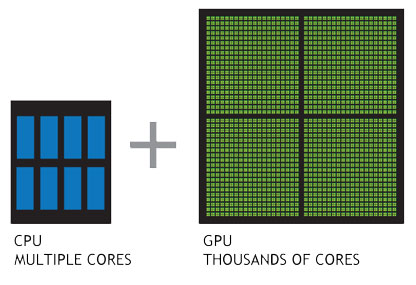
\includegraphics[width=0.4\textwidth]{cpu-and-gpu.jpg}~\cite{CPUvGPUnvidia}

A CPU has been developed from the beginning to optimize the performance of a single task. 
%
In order to accomplish this CPUs have been latency optimized, meaning that the time to complete one task, including gathering the necessary memory, has been reduced in any way possible.
%
GPUs on the other-hand have been throughput optimized in order to complete as many tasks as possible in a given amount of time.
%
This means that the time to complete a single task is most likely significantly longer than in a CPU but in a fixed amount of time the GPU will be able to accomplish many more tasks.
%
So given a large enough number of tasks that can be accomplished in parallel the GPU can complete all of them faster.



	\subsection{ \textbf{Monte Carlo Transport on a GPU}}

This section will analyze the different approaches Monte Carlo transport codes utilizing GPU architectures.
%
It will begin by comparing and contrasting different approaches by evaluating a few key areas of the studies that have been done: accuracy, performance and algorithmic choices.
%
Following will be an evaluation of the effectiveness of the approaches for the range of problems being addressed.
%
As a side note it is important to notice that speedups reported come from each paper on the hardware they were using at the time of their study; the GPU hardware has changed in computing power dramatically over the last ten years in terms of performance and additional features.

\subsection*{ \textbf{Accuracy:} }

One of the first considerations the scientific community has when being introduced to a new computing platform is what levels of accuracy can they achieve with their simulation codes.
%
Since the change from CPU to GPU computing brings a completely different hardware design it is important to understand how that design might affect the accuracy of any calculations it is performing.
%
This concern was especially important in the early days of GPU computing when double-precision was not supported and often even single-precision answers would provide slightly different results.
%
There are three key areas of accuracy to consider: Floating point precision, differences between CPU and GPU results, and IEE-754 compliance.
%

%
It was commonly assumed in the early stages of GPU computing that accuracy was lacking.
%
Many early attempts at GPU computing include discussions of accuracy in order to validate the correctness of their results.
%
While modern GPGPUs support double-precision much better than before, making much of the worry irrelevant, it is still important to consider the accuracy of a method that runs on a new hardware and may use a new algorithm.
%

\subsubsection*{\textbf{Floating Point Accuracy}}

One of the primary concerns of the early GPU studies involved understanding the limits of floating point arithmetic on the GPU architecture.
%
Nelson~\cite{nelson2009monte} describes one of his primary accuracy considerations as being the difference between single and double-precision calculations.
%
In older GPU hardware there was no support for double-precision in the hardware and so in order to achieve double-precision significantly more calculations were needed.
%
In modern GPU hardware 64 bit double-precision is becoming increasingly better supported and in the GPGPU cards there are dedicated double-precision units.
%

\subsubsection*{\textbf{Differences Between CPU and GPU results}}

An even larger concern than the differences between single and double-precision is differences in results that arise when using the same precision but on different architectures.
%
This concern can be understood by considering how floating-point math is accomplished on a computer~\cite{goldberg1991every}.
%
There are two main reasons that differences arise.
%
The first is that floating point mathematical operations performed in different orders might produce different results and, due to the nature of parallel computing, the ordering of these calculations is not guaranteed.
%
The second reason is that modern day CPUs using x86 processors perform math internally on 80 bit registers while a GPU does it on 32 bit (single-precision) or 64 bit (double-precision) registers.
%
Because of this, each math operation on a CPU might stay in registers and only be rounded down to 64 bits when it is saved to memory.
%

%
Jia et al. ~\cite{jia2010development} showed that in their development of a Monte Carlo dose calculation code they could achieve speedups of 5 to 6.6 times over their CPU version while maintaining within 1\% of the dosing for more than 98\% of the calculation points.
%
They considered this adequate accuracy to consider using GPUs for doing these computations.
%
Yepes et al.~\cite{yepes2010gpu} also considered accuracy in their assessment of their GPU implementation.
%
They concluded that, in terms of accuracy, there was a good agreement between the dose distributions calculated with each version they ran, with the largest discrepancies being only $\sim$3\%, and so they could run the GPU version as accurately as any general-purpose Monte Carlo program.
%
As these two groups have shown, this amount of error is often very small, and over the entire course of the simulation only brings 1-3\% errors.

\subsubsection*{\textbf{IEE-754 Compliance}}
Nelson discussed accuracy in his thesis work~\cite{nelson2009monte} as floating-point arithmetic accuracy was not fully IEEE-754 compliant during the time of his work.
%
Additionally, since NVIDIA has complete control over the implementation of floating point calculations on their GPUs there may be differences between generations that mitigate the usefulness of an accuracy study on one generation of hardware.
%
Current generations of the NVIDIA GPU hardware are IEEE-754 compliant however. 
%
In order to address issues of floating point accuracy they have even included a detailed description of the standard and the way CUDA follows the standard~\cite{cudaToolkitv7.5}.
So,  while floating point accuracy is still a concern, it is now no more a concern than it was on a CPU implementation.

\subsection*{\textbf{Performance:}}

Performance is a second important factor for Monte Carlo transport on GPUs.
%
Most early GPU studies emphasize their speedups over CPUs as the primary advantage for moving over to the GPU hardware.
%
Given the change in supercomputing designs these comparisons have become increasingly more important.
%

%
Often, performance is compared to the hardware maximums such as peak of FLOPS or memory bandwidth.
%
It is often assumed that an increase in available FLOPS will translate directly into incredible performance gains.
%
In Lee et al.'s Debunking the 100X GPU vs. CPU myth~\cite{lee2010debunking}, this discussion of performance is brought into new light showing the relative performance gains for different types of applications.
%
The important thing to consider is the limiting factor between the hardware and the code.
%
As a result, comparing current performance with that of peak performance is often very misleading.
%

%
The following discussions show the relative performances of Monte Carlo transport applications that either underwent a transformation to use GPUs or performed a study comparing with GPU hardware.
%
We will not see the 100x performance that is often sought after, but instead we can understand the impact that each applications problem, algorithms, and implementation differences had on the performance as a whole.
%

\subsubsection*{\textbf{Photon Transport}}
%
Badal and Badano~\cite{badal2009accelerating} present work on photon transport in a voxelized geometry showing results around 27X over a single core CPU.
%
Their work emphasizes simply using GPUs instead of CPUs as GPUs increase performance faster than CPUs.
%

%
Ren et al.~\cite{ren2010gpu} present work on photon propagation through tissue, showing around a 10X performance increase when using the GPU.
%
Their discussion expressed clearly that the performance was related strongly to the size of the data set and the number of simulated photons.
%
In addition, their results were negatively affected by high level divergence when processing different types of tissues.
%

%
Alerstam et al.~\cite{alerstam2008parallel} present work on a GPU based photon migration simulation in CUDA with speedups around 1000X over a single core CPU.
%
This specific problem does not suffer from the same divergence issues that other Monte Carlo codes have as the algorithm for completing a photon migration has very little divergence and can be easily optimized for memory layouts.
%
However, the 1000X speedup discussed here does not cover the entire application and ignores many factors that limit total speedup due to Amdahl's Law effects.
%

\subsubsection*{\textbf{Neutron Transport}}

%
Nelson's work presented in his thesis~\cite{nelson2009monte} shows a variety of models and considerations for his performance results.
%
His work solving neutron transport considered multiple models for running the problem and optimizing for the GPU.
%
The model that produced his best results shows 19X from a 49,152 neutrons per batch run for single-precision.
%
The same model shows 23X when using single-precision and fast math.
%
For double-precision performance the fastest speedups he observed were 12X.
%

Work done by Gong et al.~\cite{gong2011accelerating} in a MCNP-based application has similar performance benefits to Nelson's work.
%
Speedup factors of 16X to 23X were found depending on problem parameters.
%
This work was only an introductory attempt at implementing MCNP in CUDA, as MCNP is so large that it is time intensive to consider more than a subset of possible features and problem types.
%

Heimlich et al.~\cite{heimlich2009gpu} reported a speedup of around 15X for his neutron transport application when comparing a GPU to an 8-core CPU.
%
This work focused on optimizing a history-based approach in CUDA for the GPU and using MPI+OpenMP for the CPU.
%
This particular algorithm contained only small amounts of divergence in the code path that computes the random walk of neutrons, providing a possibility for greater use of available parallelism.
%


\subsubsection*{\textbf{Gamma Ray Transport}}
%
Work presented by Tickner~\cite{tickner2010monte} on X-ray and gamma ray transport uses a slightly modified scheme from the others by launching particles on a per block basis.
%
In this way, he hoped to remove the instruction-level dependencies between particles running on the GPU.
%
In this work, he produced speedups of up to 35X over a single core CPU, a significant improvement over similar methods launching with a particle-per-thread scheme.
%

\subsubsection*{\textbf{Coupled Electron Photon Transport}}
\label{sec:firstPassCoupledElectronPhoton}
%
Jia et al.'s  work~\cite{jia2010development} in a dose calculation code for coupled electron photon transport follows a relatively straight-forward algorithm.
%
In their work, they offload the data and computations to the GPU, simulate the particles, and then copy memory back.
%
This method produced a modest performance increase on a GPU of around 5 to 6.6X over their runs on a CPU.
%
The limitation of this speedup was attributed to the branching of the code.

\subsubsection*{\textbf{Track Repeating Algorithm}}
In contrast to Jia et al.'s work, Yepes et al.~\cite{yepes2010gpu} showed that a different algorithm could greatly improve results.
%
By converting a track-repeating algorithm instead of a full physics Monte Carlo code, Yepes et al. gained around 75X the performance on the GPU over the CPU.
%
It is thought that the simpler logic of this algorithm generated threads which followed less branching paths than the algorithm presented in Jia et al.'s work.

\subsubsection*{\textbf{Performance Evaluation}}
All of these examples contain a common theme.
%
While performance can be gained doing Monte Carlo on the GPU, it can be more difficult to get than expected due to the highly divergent nature of the Monte Carlo algorithm.
%
Methods to deal with this divergence show promising results.
%
These outcomes are expected since Monte Carlo applications are embarrassingly parallel (good for GPUs) but also incredibly divergent (bad for GPUs).
%

In this section, we have seen a wide range in performances, from as low as 5X to as high as 75X, or even 1000X.
%
While simplifications played a large role in the 75X algorithm we do see a full Monte Carlo application achieving speeds of 35X in the case of the work by Tickner~\cite{tickner2010monte}.
%
It is important to note that while some of the differences in performance are due to the nature of each problem being solved, the algorithmic choices made can have a significant impact on the GPU implementations.
%

\subsection*{\textbf{Algorithms:}}

Based on the performance studies we have just seen, it is important to highlight the algorithmic approaches that were taken so that we can understand the performance of each approach.
%
If we can clearly find algorithms that show positive performance results, then other codes can implement them for potential gain.
%
In this section, we are going to look at a few of the important algorithms.
%

%
Monte Carlo transport applications tend to follow a simple model where each tracked particle is given its own thread and computation progresses in an embarrassingly parallel fashion. 
%
On a GPU, this also makes sense as a starting point since particles are independent and this progression leads to a naturally parallel approach.
%
It is often pointed out, however, that due to the divergent nature of Monte Carlo this approach might not be the best way organize Monte Carlo codes on GPU hardware.
%

\subsubsection*{\textbf{Particle-Per-Block}}
We will first look at an alternative approach, the particle-per-block tracking algorithm described by Tickner~\cite{tickner2010monte}.
%
First each tracked particle or quantum of radiation is given to a block of threads.
%
Then calculations are performed for one particle on each block of threads.
%
For example the particle intersection tests with the background geometry can be performed in parallel on those threads for each piece of geometry that particle might be able to collide with.
%
Areas where these parallel instructions can be utilized within a particle's calculation are then used by the threads in a block computing for that particle.
%

This particle-per-block technique is effective in mitigating the divergence issue.
%
Particles often diverge quickly from one another in the code paths they follow.
%
This means that threads in a block are not always able to travel in lock step and can cause some serialization of the parallel regions.
%
By using only one particle per block, the divergence problem is nearly removed from the equation.
%
Additionally, this method introduces a new area of parallelism that is not otherwise being taken advantage of: instruction-level parallelism in the calculations for a single particle.
%

%
This method, however, does not take full advantage of the parallelism in the hardware like the methods that are not sensitive to divergence.
%
Many threads can execute simultaneously within a block with potential slowdowns coming from when groupings of 32 threads are held in a warp and forced into the lockstep pattern.
%
Running only one particle per block can sacrifice some parallelism, as not all tasks to calculate a particle's path are parallel operations.
%
Additionally, since warps are scheduled out of thread blocks, any particle operations that are not done in parallel among the threads of a block are serializing themselves in a similar manner as to those algorithms that run one thread per particle and contain high levels of divergence.
%

In summary, this method has some merit if it can find enough parallel work in the thread block to execute additional parallel tasks that would otherwise be stalled when following a simpler method.
%
Also, this method might end up showing the same characteristics of the simpler particle-per-thread model if the extra parallelism is not found, and instead lose out on the parallelism provided by particles that are not highly divergent from one another. 

\subsubsection*{\textbf{Event-Based Approaches}}

A second, possibly more obvious method, to escape the divergence issue is to switch particle tracking algorithms more dramatically from a history based version to an event based version.
%
Section~\ref{sec:EventBased} discusses this topic later in this paper.
%
Event based approaches require much more work then simply transforming an existing code to use the history based version on the GPU.
%
And as Du et al. discovered in their attempt at an event based Monte Carlo version of the Archer code~\cite{xu2015archer}~\cite{du2013evaluation}~\cite{liu2015comparison}~\cite{su2013monte},  getting any speedups with that method creates a whole new host of challenges to overcome: divergence, atomic operations, data locality/layouts, and portability to name a few.

\subsubsection*{\textbf{Voxelization Approaches}}

This method was used for comparing workloads on GPUs and is often done to voxelize geometries to enable Monte Carlo codes to run.
%
Voxelization of a geometry is done on a voxel-by-voxel basis.
%
This process involved ray-stabbing numbers counted on the GPU, and then using a parity-counting method on the CPU to detect if the voxel was inside the mesh surface~\cite{na2010deformable}.
%
This method contains no divergence since all threads follow the exact same code paths.
%
Doing this algorithm with no divergence produces a 45.5x speedup on the GPU over the CPU.
%
This example is in Ding et al.'s evaluation report~\cite{ding2011evaluation} in order to show the performance of the same GPU on different aspects related to Monte Carlo transport.

\subsection*{ \textbf{Evaluation:}}

\begin{table}
\caption { GPU speedup evaluation results~\cite{ding2011evaluation} } \label{tab:GPUPerfEval} 
\begin{center}
\begin{tabular}{ |C{.10\textwidth}|C{.10\textwidth}|C{.10\textwidth}|C{.10\textwidth}|}
\hline
 & & & \\
Case & Execution Time $T_{CPU}$ (minutes) & Execution Time $T_{GPU}$ (minutes) & Speed-up Factor $T_{CPU}/T_{GPU}$ \\
 & & & \\
 \hline
 & & & \\
Neutron Transport Problem & $~ 0.496$ & $ ~0.017$ & $~ 29.2$ \\ 
 & & & \\
\hline
 & & & \\
Eigenvalue/Criticality Problem & $ 4.25 $ & $ ~ 0.5 $ & $ ~ 8.5 $ \\
 & & & \\
\hline
 & & & \\
Voxelization & $ 2380.4 $ & $ ~ 52.3 $ & $~ 45.5 $ \\
 & & & \\
\hline
\end{tabular}
\end{center}
\end{table}

A number of studies were conducted by groups identifying the potential benefits of GPU hardware but also software development issues with Monte Carlo applications. 
%
Among these concerns are memory limitations, lack of ECC support, lack of software optimization, limitations of SIMD architecture, clock speeds, and complex memory allocation schemes.
%
In addition, the achieved performance often did not exceed that of unchanged codes on a cluster.
%
In some cases, though, speedups were large and easy to achieve, such as the 45X speedup of the voxelized approach. 
%
The results from Ding et al.'s~\cite{ding2011evaluation} evaluations can be seen in Table~\ref{tab:GPUPerfEval}.
%
The only strong conclusion from these works are that a clear and defined path are not yet known on how to take full advantage of the available parallelism without suffering performance penalties in turn.

	\subsection{\textbf{Monte Carlo and Medicine}}

A perspective of Monte Carlo transport that often gets overlooked by others in the field is the area of Monte Carlo transport for medicine.
%
Radiation transport calculations are used for dose estimations in patients and require close to real time, highly accurate solutions on desktop style machines.
%
The following are descriptions from three applications of medical Monte Carlo transport followed by an evaluation of the effect GPUs have had on the field.

\subsection*{ Electromagnetic Monte Carlo transport in GMC}

Janhnke et al. ~\cite{jahnke2012gmc} in 2012 described his groups efforts to develop the code named GPU Monte Carlo (GMC).
%
GMC is a GPU implementation of the low energy electromagnetic portion of the Geant4 code using the CUDA interface.
%
GMC runs in a thread per particle style operating on 32768 particles at a time (128 blocks of 256 threads).
%
GMC runs through a series of kernel launches in a loop each handling one important aspect of the physics.

The raw performance differences between the CPU version and the GPU implementation for the problems tested is amazing for this problem.
%
The average for their study showed the GMC histories being computed at a rate of 657.60 histories every milli-second compared to the Geant4 CPU with histories computed at 0.137 histories per milli-second.
%
Comparing these two numbers produces a speedup factor of 4860 while maintaining reasonable accuracy in all cases between CPU and GPU with accuracies greater than 95\% in all regions.
%
Total runtimes were also brought down to the hundreds of seconds showing the possibility for clinical usage of applications like this.~\cite{jahnke2012gmc}

\subsection*{ Proton Therapy in gPMC}

Accurately computing radiation doses is a critical part of proton radiotherapy, and Monte Carlo simulations are considered to be the most accurate method to compute those dose calculations.
%
Given the long time required for traditional applications to use this technique, clinical application have been severely limited.
%
Jia et al.~\cite{jia2012gpu} describes a fast dose calculation code, gPMC, and how it might enable clinical usage of Monte Carlo proton dose calculations.

%
The code gPMC was developed in CUDA for use on a GPU.
%
Using a batching system to launch groups of particles from a particle stack.
%
gPMC runs for between 6 and 22 seconds to generate passing rates between 95\% and 99\%.
%
The authors except that they have successfully developed a dose calculation code under a certain set of restrictions and are hopeful that their future work will be able to meet with continuing success as they expand the context for their application.~\cite{jia2012gpu}

\subsection*{Electron-Photon Transport in DPM }

Jia et al.~\cite{jia2010development} describes the development of a CUDA based Monte Carlo coupled electron-photon application for dose planning, called DPM (dose planning method).
%
 Their scheme involves launching a kernel on the GPU that simulates all of the particle histories necissary to reach some target number of source particles.
 %
 Each thread of their kernel simulates the history of one source particle and all secondary particles that it generated.
 %
 The kernel ends with an atomic gathering of all the dosing data.
 %
 DPM was only able to achieve speedups of around 5-6.6x on the GPU over the CPU, but did get excellent agreement on relative uncertainties in their results.~\cite{jia2010development}
 
 Jia et al.~\cite{jia2011gpu} revisits their DPM code and is able to change speedups of 5-6.6x into speedups of approximately 69 - 87x.
%
DPMs main algorithm changed in a few significant ways.
%
First a single thread only computed the history of a single particle and any additional particles were placed on a stack for a future iteration.
%
Secondly the photon and electron physics was separated into different kernels so that threads would experience less divergence when handling the necessary code paths.
%
Other factors such as a better random number generator and use of the hardware linear interpolation features were also done.
%
With the additions of new features and improvements, DPM re-evaluated their accuracy to be not statistically significant in over 96\% of regions for all problems they tested.
%
Given the now excellent speedups of 69-87x and acceptable accuracy ranges, real time speeds for realistic problems was achieved.
~\cite{jia2011gpu}


\subsection*{Evaluation}

These three projects show a variety of problems in the medical Monte Carlo field.
%
They are each accomplishing their tasks on a single GPU as opposed to a cluster of CPUs.
%
There are numerous stated benefits to this, cost of purchasing and operating a cluster against purchasing a single GPU being a large factor.
%
In each case speedups were achieved that were adequate to bring the time if their simulations down to those that would be useful in a clinical environment.
%

	\subsection{\textbf{Monte Carlo and Ray Tracking}}

One important and often computationally expensive aspect of Monte Carlo transport is the step that determines if the particle will collide with any background geometry, or at least cross into a zone of a different material.
%
This is done through a similar method as that used in ray tracing.
%
Ray tracing is a technique in computer graphics for ``generating an image by tracing the path of light through pixels in an image plane and simulating the effects of its encounters with virtual objects"~\cite{wikipediaRayTracing}.

The general process of ray tracing is very similar to Monte Carlo transport in the need to do many intersection tests from potentially scattered sources.
%
Bergmann decided to study the potential of using the power of a highly optimized GPU ray tracing library, OptiX~\cite{2014development}.
%
OptiX is a scalable framework for building ray tracing applications~\cite{optixProgrammingGuide}~\cite{parker2010optix}.

%
The first study conducted was to determine the optimum configuration for OptiX as well as the capability for OptiX to be initialized with random starting points and directions as is most likely to be the case in a Monte Carlo application.
%
When using a ray tracing library it is important to consider the two areas that can scale: the number of concurrently traced rays and the number of geometrical objects in the scene.
%
Nuclear reactor simulations might contain thousands of material zones in complex geometric layouts; knowing this last scaling parameter is especially important to not overlook~\cite{2014development}.
%
In these studies, the rates became fairly consistent after reaching $10^6$ particles.
 %
Bergmann also notes some important points, such as which acceleration structure was always best and when memory become a constraint on the problem that could be run.
 %
 The conclusion from this study was that OptiX could be used to handle the geometry representation in a Monte Carlo neutron transport code.
 %
 Additionally, for best performance one should use a primitive-based geometry instancing method, a BVH acceleration structure, and run as many parallel rays as possible.
%

%
In addition to the use of a pre-existing tool like NVIDIA's OptiX library, other groups looked at optimizing Monte Carlo transport by focusing on treating it like a ray tracing problem.
%
Xiao et al.~\cite{xiao2015monte} focused on the data locality issues in all ray tracing applications on GPUs.
%
They describe a new data locality method based on task partitioning and scheduling in order to enhance spatial and temporal data locality by ordering random rays into coherent groups.
%
By applying this method they achieved a 6-8X speedup over the previous GPU version of radiation therapy Monte Carlo transport. 
%
Despres et al.~\cite{despres2008stream} studied the ray tracing algorithm for tracing a path through a grid in the context of Monte Carlo applications.
%
Their GPU implementation of the Suddon algorithm, showed a speedup factor of 6X over the CPU.
%
This work provides context for an important portion of the Monte Carlo transport problem, a look at the transport piece itself.
%

%
These examples show that progress in connected fields can positively impact the approaches in Monte Carlo transport.
%
Ray tracing is only one aspect of a full Monte Carlo transport application but as it can be greatly beneficial to look at work done in these related fields and bring those ideas back into the full application.


	\subsection{\textbf{Event-Based Techniques}}
\label{sec:EventBased}

Much discussion has been aimed at the negative effect divergence in Monte Carlo codes has on  performance.
%
Given the embarrassingly parallel nature of the Monte Carlo transport algorithm, performance of Monte Carlo transport codes on the GPU should be incredible.
%
This survey has shown however, that the opposite is often seen in practice.
%
Many applications achieve only marginal speedups, siting that the cause of their lack in performance was due to divergence in the code.
%

%
In order to combat divergence, an old scheme was re-evaluated for use on GPU architectures.
%
Given some of the similarities between the classic vector machines of the 1980's/90's with modern GPU hardware, it is reasonable to consider some of those algorithms for use now.
%
In particular, the event-based approach worked well on SIMD vector hardware.
%
In the event-based approach particles are processed in groups which perform the same event.
%
There are multiple variations to this idea, a few of which are presented here.
%

\subsection*{\textbf{Vectorized Algorithm}}

%
Early event-based algorithms were designed for vector machines and were called vectorized algorithms.
%
Martin describes a successful vectorized algorithm as well some variations in his paper~\cite{martin1989successful}.
%
The conventional Monte Carlo algorithm cannot be vectorized since treating many histories simultaneously would immediately fail after the first step of the simulation as each particle can undergo a different event.
%
In order to achieve vectorization the histories need to be split into events, which are similar and can be processed in a vectorized manner, i.e., the same set of instructions.
%
The basic event-based iteration algorithm is described in Algorithm~\ref{alg:basicEvent}.
%

%
\begin{algorithm}
\DontPrintSemicolon
\caption{The basic iteration event}
\label{alg:basicEvent}
\For{ event n = 0, 1, 2, ... }
{
	 Fetch $\Gamma^{n}$ \\
	 Preform free flight analysis:\\
	\Indp	 gather the cross section data and geometry data tabulated by particle,\\
		 $\Sigma \leftarrow$ S,\\
		 $\rho \leftarrow$ R;\\
		 using $\Sigma$, sample a vector of distances to collision, $d_{c}$\\
		 using $\rho$, determine vector of minimum distances to boundary, $d_{b}$\\
		 determine the minimum distances to the end of event,\\
		\Indp $d_{min}$ = min[$d_{c}, d_{b}$];\\
		\Indm  update the particle coordinates,\\
		\Indp $r^{n+1}$ = $r^{n} + \Omega^{n} \cdot r_{min}$\\
	\Indm  Perform collision analysis:\\
	\Indp  gather particle attributes,\\
	\Indp $\Omega \leftarrow \Gamma^{n}, E \leftarrow \Gamma^{n}$;\\
	\Indm  evaluate collision physics for new direction cosines and energies,\\
	\Indp $\Omega ' \leftarrow \Omega$, $E' \leftarrow  E$\\
	\Indm  scatter new particle attributes back into bank,\\
	\Indp $\Omega ' \leftarrow \Gamma^{n}$, $E' \leftarrow  \Gamma^{n}$\\
	\Indm \Indm  Perform the boundary analysis:\\
	\Indp  gather particle zone indices $Z$,\\
	\Indp $Z \leftarrow \Gamma^{n}$\\
	\Indm  determine new zone indices,\\
	\Indp $Z' \leftarrow Z:$\\
	\Indm  scatter new zone indices back into bank.\\
	\Indp $Z' \rightarrow \Gamma^{n}$\\
	\Indm \Indm  Update the particle bank,\\
	\Indp $\Gamma^{n} \Rightarrow \Gamma^{n+1}\ (with\ L_{n+1}\ particles )$ \\
	(e.g. compress out terminated particles).\\
	\Indm  If $L_{n+1} \neq 0, continue$\\
%	\State using \Sigma, sample a vector of distances to collision, $d_{c}$
%	\EndIndent
}
\end{algorithm}
%

In addition to the basic event-based approach there are a few variations discussed in Martins paper that expand on this model.
%
One variation is the stack-driven approach.
%
In this approach the events are further divided into smaller computational tasks.
%
Instead of cycling through the tasks in a fixed order, the computation can move forward by selecting the event with the largest number of particles.
%
This involves a tradeoff of simplified control flow versus maximizing the vector lengths of the computational components.
%

In recent work by Ozog et al.~\cite{ozog2015performance}, multiple approaches to vectorization were tried.
%
The banks of particles method described in Ozog et al.'s paper follows the same form as the original basic stack based algorithm, with sub-stacks to manage vectorizable groupings of particles.
%
A second idea, that offered performance benefits of 1.6x for an Intel many integrated core (MIC) processor over an Intel Xeon processor, was to vectorize nuclear data lookup portions of the code.
%
In this way particles are processed in the same history based manner (little to no code changes required), and vector units are utilized to preform the expensive nuclear data lookup and interpolation calculations.

%
Vectorized versions of the Monte Carlo transport algorithms are generally based on this original basic algorithm.
%
There are many variations but the principal differences all depend on the methods used for organizing and treating the vectors of particles.
%
There are variations using stacks, tags, and tasks.
%
When wishing to change an existing history-based legacy code, the major downside to the event-based approach is that it requires a large change to pre-existing source code.
%

\subsection*{\textbf{Event-Based for GPU}}

%
Event-based methods used for the GPU follow similar design patterns as those that were developed for vector machines.
%
One prime example is the event-based version developed by Bergmann for the code WARP~\cite{2014development}.
%
Figure~\ref{fig:innerLoopWARP} outlines the inner transport loop broken into its separate stages.
%
Figure~\ref{fig:outerLoopWARP} outlines the outer transport loop between neutron batches.
%

\begin{figure}
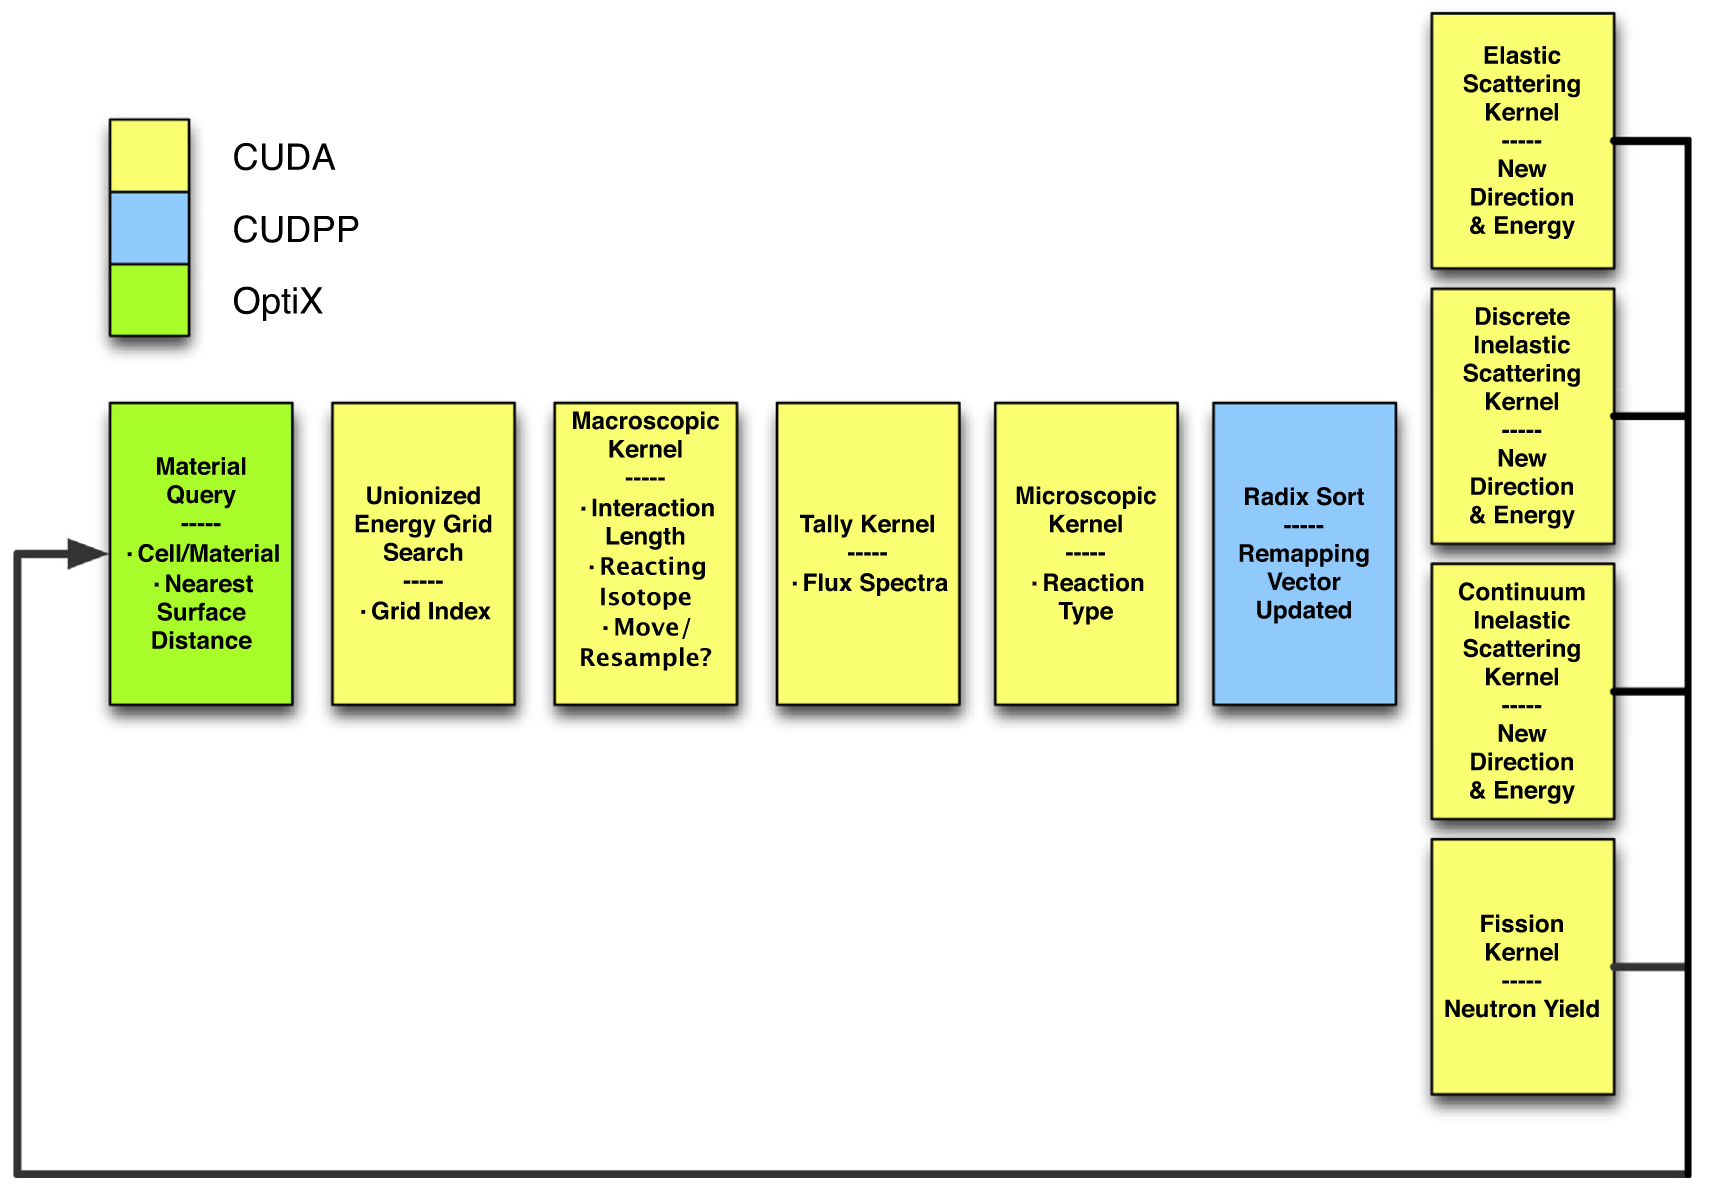
\includegraphics[width=0.49\textwidth]{InnerLoopWARP}
\caption{WARP inner tranport loop that is executed until all neutrons in a batch are completed~\cite{2014development}}
\label{fig:innerLoopWARP}
\end{figure}

\begin{figure}
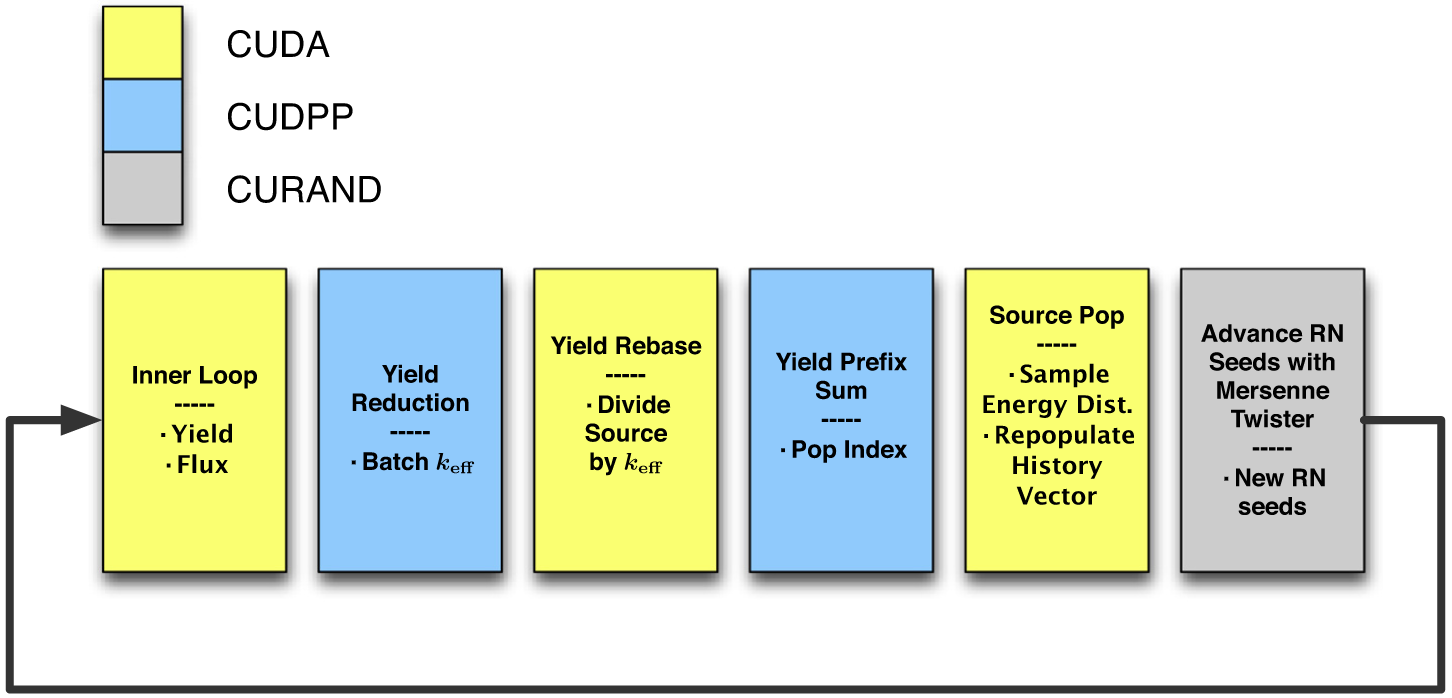
\includegraphics[width=0.49\textwidth]{OuterLoopWARP}
\caption{WARP outer transport loop that is executed in between neutron batches for criticality source runs~\cite{2014development}}
\label{fig:outerLoopWARP}
\end{figure}

Bergmann utilizes a series of kernels that each solves one piece of the process.
%
Once each neutron knows which path it will go down -- i.e. scattering, fission, etc. -- each of those possible paths is launched in a separate kernel.
%
Unlike the basic vectorized approach or the stack based approach however, all of the events are launched at once using concurrent kernels due to CUDA streaming properties.
%
In this way, the main divergent part of the code is broken into relatively non-divergent kernels which are then launched simultaneously so as to continue to utilize the full hardware.

Not all attempts at vectorization, or implementing an event-based algorithm for Monte Carlo transport codes, have been successful.
%
Liu~\cite{liu2014comparative} describes an event-based approach that after being implemented produced a roughly ten times slower version then the history-based code.
%
This example shows how complicated the task of implementing an event-based algorithm can be, and that it is possible as well that not all Monte Carlo transport problems can be solved efficiently in an event-based fashion.
%
Liu attributed their slow down to the memory access latency due to the high amount of global memory transactions and showed that the cost of this in an event-based method did not outweigh the benefit of reducing thread divergence and increasing warp execution efficiency.







\section{\textbf{What is Portable Performance}}

The term portable performance generally means the ability to achieve a high level of performance on a variety of architectures.
%
In this case high performance is relative to each target system~\cite{michaelwolfe2016}.
%
One important consideration then is what variety of systems are used that applications need to be portable for. 
%

%
The top ranked machines in the world currently utilize technologies like general purpose graphics processing units (GPUs, e.g., NVIDIA Tesla in Titan ), many-core co-processors (e.g., Intel Xeon Phi in Tianhe-2), and large multi-core CPUs (e.g., IBM Power, Intel Xeon in Tianhe-2 and others)~\cite{michaelwolfe2016},~\cite{top500thelist2016},~\cite{hankchilds2015}. 
%
Further, future supercomputing designs may include low-power architectures (e.g., ARM), hybrid designs (e.g., AMD APU), or experimental designs (e.g., FPGA systems)~\cite{hankchilds2015}. 
%
Given this wide array of possible architectures the value of portable performance has never before been so high.
%

\subsection{ \textbf{Abstraction Layers}}


\subsection*{\textbf{OpenMP}}

Parallelism through OpenMP is achieved through the use of compiler directives, library routines, and environmental variables.
%
These are used to specify the high level parallelism for programs using the Fortran and C/C++ languages.
%
These directives, routines and variables have been expanded to include methods to describe regions of code or data should be moved to another computing device, like an accelerator.~\cite{openmp}

Lee et. al.~\cite{lee2009openmp} describe several advantages for using OpenMP as a programming paradigm for use on a GPGPU:
\begin{itemize}
\item "OpenMP is efficient at expressing loop-level parallelism in applications, which is an ideal target for utilizing GPU's highly parallel computing units to accelerate data-parallel computations.
\item The concept of a master thread and a pool of worker threads in OpenMP's fork-join model represents well the relationship between the master thread running on the host CPU and a pool of threads in a GPU device.
\item Incremental parallelization of applications, which is one of OpenMP's features, can add the same benefit to GPGPU programming."
\end{itemize}~\cite{lee2009openmp}

By including target device directives as well as other supporting features, OpenMP is able to utilize its experiences in parallel computing and offer a familiar solution to programmers who need to make new or existing algorithms and codes work for parallel CPUs, GPUs and more.
\cite{ayguade2010extending}

\subsection*{\textbf{OpenACC}}

OpenACC enables the offloading of loops and regions of code onto accelerator devices.
%
The OpenACC API uses a host-directed model of execution where the main program runs on the host, or CPU, and the computational work is offloaded to a device accelerator, or GPU.
%
The OpenACC memory model outlines two memory spaces which do not automatically synchronize, requiring explicit synchronization calls between memory spaces.
%
OpenACC operates in a similar fashion to OpenMP by using compiler directives to define regions of code for their operations to effect.
\cite{wienke2012openacc}

OpenACC is designed to be portable.
%
Its directive based programming allow programmers to create high-level host+accelerator applications without needing to explicitly handle many of the extra aspects to working on an accelerator.
\cite{openacc}

OpenACC has shown to be able to achieve reasonable performance on multiple platforms.
%
Wang et. al.~\cite{wang2013performance} performed a performance study showing that for some benchmarks the OpenACC version were able to achieve more than 82\% performance when compared with peak performance for both the Intel Knights Corner and NVIDIA Kepler architectures.

\subsection*{\textbf{Thrust}}

Thrust is a library of algorithms and data structures that can be used to provide an interface to parallel programming in order to increase a programmers productivity.
%
Thrust is designed similar to the standard template library, allowing programmers familiar with the C++ STL to feel instantly comfortable working in the thrust environment.
%
Through this design pattern Thrust has lowered the barrier to entry allowing access to GPU hardware and memory without the needed to interact with the CUDA API.
%
\cite{hoberock2010thrust}

In addition to adding parallel algorithms, Thrust provides multiple compilable backend technologies that allow the programmer to write their algorithms using thrust and then compile them in CUDA, TBB, and OpenMP.
%
This offers up a wide array of portable solutions that programmers can take advantage of in order to much more easily write portable and performant applications.
\cite{thrust}

Thrust offers a variety of algorithms with significant performance advantages leading to real world performance gains.
%
Such as upwards of 32x performance gains over niave algorithm implementations of the fill algorithm on some hardware, and 2.7x performance gains with radix sort by utilizing only significant bits when possible.
%
These performance gains come for free when using a thrust algorithm to accomplish a data parallel task.
%
~\cite{bell2011thrust}

In addition, thrust provides all of the main data parallel operations defined in Guy Blellochs work~\cite{blelloch1990vector}.
%
One method of achieving performance is to then rewrite an algorithm using data parallel primitives or algorithms and then use the existing Thrust methods to preform the operations.

\subsection*{\textbf{RAJA}}

The RAJA portability layer is designed to be a lightweight method of providing loop-level parallelism in existing codes.
%
The idea behind the design was that, especially at labs like LLNL, there are a large number of scientific code basis that will need to make some sort of transition in order to utilize upcoming architectures.
%
RAJA was designed to be able to replace curretly existing loops with with a wrapper loop to at first make no change or impact; but then
%
once the RAJA abstraction layer is in place, the loop can be changed to run on different architectures.
%
\cite{hornung2014raja}
\cite{hornung2016raja}

RAJA achieved their flexibility through macro replacements in the library.
%
By changing a compile time option the user can define if they want the OpenMP parallel launcher, a CUDA kernel launcher, or a serial launcher.
%
In this manner RAJA is a useful tool for generically replacing large numbers of parallel loops with a consistent theme that creates inlined parallel code for the compilers to optimize, instead of the large and sometimes convoluted template models.
%
\cite{hornung2014raja}
\cite{hornung2016raja}

In addition to providing a library, the RAJA group provided an idea for a second possible approach to portability.
%
RAJA like approaches involve custom macro definition to replace the variable portions of the code inline and offer the compiler the path it expects, while minimizing code redundancy when programming for multiple platforms.

\subsection*{\textbf{Kokkos}}

The Kokkos C++ library provides a programming model that enables performance portability accross devices.
%
The objective of the Kokkos library is to allow as much of the users code as possible to be compiled for different devices, while obtaining the same performance as a variant of the code that was written specifically for that device.
%
Kokkos uses the idea of execution and memory spaces to provide an abstraction to the problem.
%
In their model threads are said to execute in an execution space, while data resides within a memory space.
%
Then relationships are defined between the different execution and memory spaces.
\cite{edwards2014kokkos}

Parallelism in Kokkos comes from parallel execution patterns, data parallel and task parallel patterns are used.
%
The primary data parallel patterns are: parallel\_for, parallel\_reduce, and parallel\_scan.
%
The data parallel computational kernels are implemented as standard c++ functors.
%

The Kokkos abstraction layer has demonstrated performance of approximately 90\% of the performance of the optimized architecture specific versions for kernel tests and mini-applications.
%
Kokkos has demonstrated performance on Xeon, Xeon Phi, and Kepler architectures, showing the portability of this solution.
\cite{edwards2014kokkos}
\cite{edwards2012manycore}

\subsection*{\textbf{Chapel}}

Chapel is an object-oriented parallel programming language which was designed from first principles~\cite{sidelnik2012performance}.
%
Chapel was developed in order to improve the programmability and productivity of development on parallel machines.
%
DARPA's High Performance Computing Systems defines productivity as "a combination of of performance, programmability, portability, and robustness".
~\cite{chamberlain2007parallel}
%
Chapel used this idea to make a global-view parallel language that uses a block-imperative programming style.
%
Chapel purposely avoided building on the C or Fortran languages in order to help programmers avoid falling back into sequential programming patterns.
%
\cite{chamberlain2007parallel}

Chapel uses a code generation design to generate parallel C or CUDA code.
%
The Chapel language defines the parallelism and so can be used as the basis for optimized code generation on many different platforms.
%
Chapel uses this design to achieve portability and performance with their language.

Chapel's design goal is to support any parallel algorithm that a programmer could conceive without the need to fall back to other parallel libraries.
%
Chapel supports concepts for describing parallelism separate from those used to describe locality.
%
It supports programming at higher and lower levels, as required by the programmer as well as advanced higher-level features such as data distributions or parallel loop schedules.
%
~\cite{bradchamberlain2013}


\subsection*{\textbf{VTK-m}}

VTK-m arose as the joined collaborations of three separate groups at three separate national labs combining together and joining forces with Kitware, the owners of the current VTK (Visualization ToolKit) software.
%
Visualization applications use VTK in order to express visualization algorithms and data structures in their codes.
%
VTK-m came about from the three projects, EAVL, DAX, and PISTON, with the design goal of being a portable performance solution for visualization applications and algorithms.
%

The VTK-m framework takes the concepts of data parallel primitives and patterns generated from those primitives to provide a framework for accomplishing visualization algorithms.
%
By utilizing data parallel primitives that can be compiled for different platforms, VTK-m achieves portable performance.
% 
\cite{moreland2015vtk}
\cite{moreland2014vtk}

The contributions of the three projects to VTK-m are as follows.

\begin{itemize}
\item[EAVL] Provided a robust data model
\item[DAX] Provided a model for parallel work dispatching
\item[Piston] Provided many data parallel algorithms and implementations
\end{itemize}

\subsubsection*{\textbf{EAVL}}

EAVL or the Extrame-scale Analysis and Visualization Library was developed with three goals in mind: Data Model -- "Expanding on traditional models to support current and forthcoming scientific data sets". Efficiency -- "Improve memory and algorithmic efficiency through the enhanced data model, and support stricter memory controls and accelerator device memory models". Scalability -- "Support distributed and data parallelism, and transparently target heterogeneous systems."
~\cite{jeremyEAVL}

\subsubsection*{\textbf{Dax}}

Dax or Data Analysis at Extreme is a library developed to support fine grained concurrency for data analysis and visualization algorithms.
%
This toolkit provides a dispatcher that schedules worklets onto data.
%
The Dax toolkit simplifies the development of parallel visualization algorithms and provides a data parallel framework for scheduling and launching parallel jobs.
~\cite{morelanddax}
~\cite{moreland2011dax}

\subsubsection*{\textbf{PISTON}} 

The Portable Data-Parallel Visualization and Analysis Library, referred to as PISTON, is a cross-platform library that provides operations for scientific visualization and analysis.
%
These operations are preformed using data parallel primitives and the NVIDIA Thrust library.
%
PISTON uses Thrust to preform the data parallel operations and for its cross-platform compatibility.
%
PISTON adds useful algorithms for data visualization and analysis as well as an interface into the thrust calls.
~\cite{PISTON}


\section{\textbf{Monte Carlo and Portable Performance}}

In this section Monte Carlo transport applications will be evaluated as a platform for portable performance studies.
%
Monte Carlo transport offers a unique set of challenges and interesting lessons when evaluating portable performance possibilities.
%
Efforts in Ray Tracing using the EAVL/VTK-m framework showed significant success and provide workloads that are similar to those used in Monte Carlo transport problems.
%
In addition, the idea of portable performance is popular with many different groups, who are putting forward possible designs and library options.
%
Each of these designs or abstraction layers-- EAVL, DAX, PISTON, VTK-m, Thrust, OpenMP, OpenACC, RAJA, Chapel, and Kokkos --has its own pluses and minuses, as well as requiring different amounts of effort in order to make it function within already existing codes.
%

%
There is a large number of potential directions and possible areas to focus on in this study.
%
Looking now at Bleile's work with a Monte Carlo mini app, ALPSMC~\cite{alpsmc1}~\cite{alpsmc2}, the Monte Carlo algorithmic question of event based versus history based algorithms in a simplified Monte Carlo code was evaluated.
%
In addition, the effects that different parallel paradigms have on performance as well as the ease of code conversion were studied.
%

\subsection{\textbf{ALPSMC}}

ALPSMC~\cite{brantley2011benchmark} is a Monte Carlo test code that models neutron transport in a one dimensional planar geometry, through a binary stochastic medium.
%
It is originally a serial C++ application that follows an all particle history based approach.
%
This history based algorithm is shown in Algorithm~\ref{alg:history-based}
%

\begin{algorithm}
\DontPrintSemicolon
\caption{History-based Monte Carlo algorithm}
\label{alg:history-based}
\ForEach{particle history}
{ 
    generate particle from boundary condition or source\;
    \While{particle not escaped or absorbed}
    {
       sample distance to collision in material\;
       sample distance to material interface\;
       compute distance to cell boundary\;
       select minimum distance, move particle, and perform event\;
       \If{particle escaped spatial domain}
       {
          update leakage tally\;
          end particle history\;
       }
       \If{particle absorbed}
       {
          update absorption tally\;
          end particle history\;
       }
    }
}
\end{algorithm}
%

%
The original work was to convert this algorithm into an event based approach.
%
The event based algorithm performs data parallel operations across all of the particles that are in the same event, as well as a series of data parallel steps required to do proper book keeping to get the particles for each event.
%
The event based algorithm is defined in Algorithm~\ref{alg:eventbased}.
%
The operations required to launch the event kernels are defined as follows and correspond to lines 6 and 7 of Algorithm~\ref{alg:eventbased}.
%
\begin{itemize}
\item{[Step 1:]} thrust::transform --- Fill out a stencil map of 1's and 0's of all particles doing event E (where each particle whose next event is E will get a 1 in the stencil map at its index location)
\item{[Step 2:]} thrust::reduce --- Count the number of elements labeled 1 in the stencil (determines the number of particles that will perform event E)
\item{[Step 3:]} Check if the number of elements is greater than 0 (check if any particles are performing event E)
\item{[Step 4:]} thrust::exclusive\_scan --- generate indices for index mapping from stencil map (indices for each particle performing event E)
\item{[Step 5:]} Allocate a new map of appropriate size (map to hold indices for all particles performing event E)
\item{[Step 6:]} Scatter indexes from scan into new index map (reduces the exclusive\_scan generated indices into the map that holds only enough for particles performing event E)
\item{[Step 7:]} Use new index map in permutation\_iterator loops over all particles (combining the index map with the permutation iterator allows loops over all particles to operate only on the particles selected in the index map)
\end{itemize}
~\cite{alpsmc1}
%

\begin{algorithm}
\DontPrintSemicolon
\caption{Event-based Monte Carlo algorithm}
\label{alg:eventbased}
\ForEach{batch of particle histories (fits in memory constraint)}
{ 
    generate all particles in batch from boundary condition or source\;
    determine next event for all particles (collision, material interface crossing, cell boundary crossing)\;
    \While{particles remaining in batch}
    {
       \ForEach{event E in (collision, material interface crossing, cell boundary crossing)}
       {
          identify all particles whose next event is E\;
          perform event E for identified particles and determine next event for these particles\;
       }
       \If{particle escaped spatial domain}
       {
          update leakage tally\;
       }
       \If{particle absorbed}
       {
          update absorption tally\;
       }
       delete particles absorbed or leaked\;
    }
}
\end{algorithm}

Thrust was chosen as the platform for implementing the data parallel operations, though many of the options discussed would have worked for this.
%
The key design choice was that each operation can be done using data parallel primitives.
%
This study also use a direct CUDA implementation that launched kernels for the main events and used Thrust for data management for comparison.

The performance results from the initial implementation~\cite{alpsmc1} were varied, with the best CUDA version reaching about 12x and the thrust OpenMP version reaching 2.2x with 16 threads.
%
The optimized implementation discovered a few areas for improvement and achieved fairly significant results.
%
Table~\ref{tab:ALPSspeedup} shows the summary of ALPSMC speedup results~\cite{alpsmc2}.
%

\begin{table}
\caption { Maximum speedups for each approach when compared to the original history-based serial method } \label{tab:ALPSspeedup} 
\begin{center}
\begin{tabular}{ |c|c|}
\hline
Method & Speedup\\
\hline
CUDA Event SOA & 31.32\\
\hline
CUDA History & 52.78\\
\hline
Thrust Event CUDA SOA & 54.62\\
\hline
Thrust Event OpenMP SOA & 5.54\\
\hline
\end{tabular}
\end{center}
\end{table}

Through this experience we have demonstrated a few important points.
%
First we demonstrated excellent performance in both algorithms, achieving \textasciitilde50x performance for both history and event based algorithms.
%
Additionally, these examples showed that using data parallel design and an abstraction layer -- in this case Thrust -- can preform just as well as when programmed in native CUDA under some circumstances. 
%
Lastly, while the GPU performance is high the CPU performance is still lacking.
%
Figure~\ref{fig:OMPScale} shows that the OpenMP version scales well but it has a much higher overhead than the original serial version.

\begin{figure}
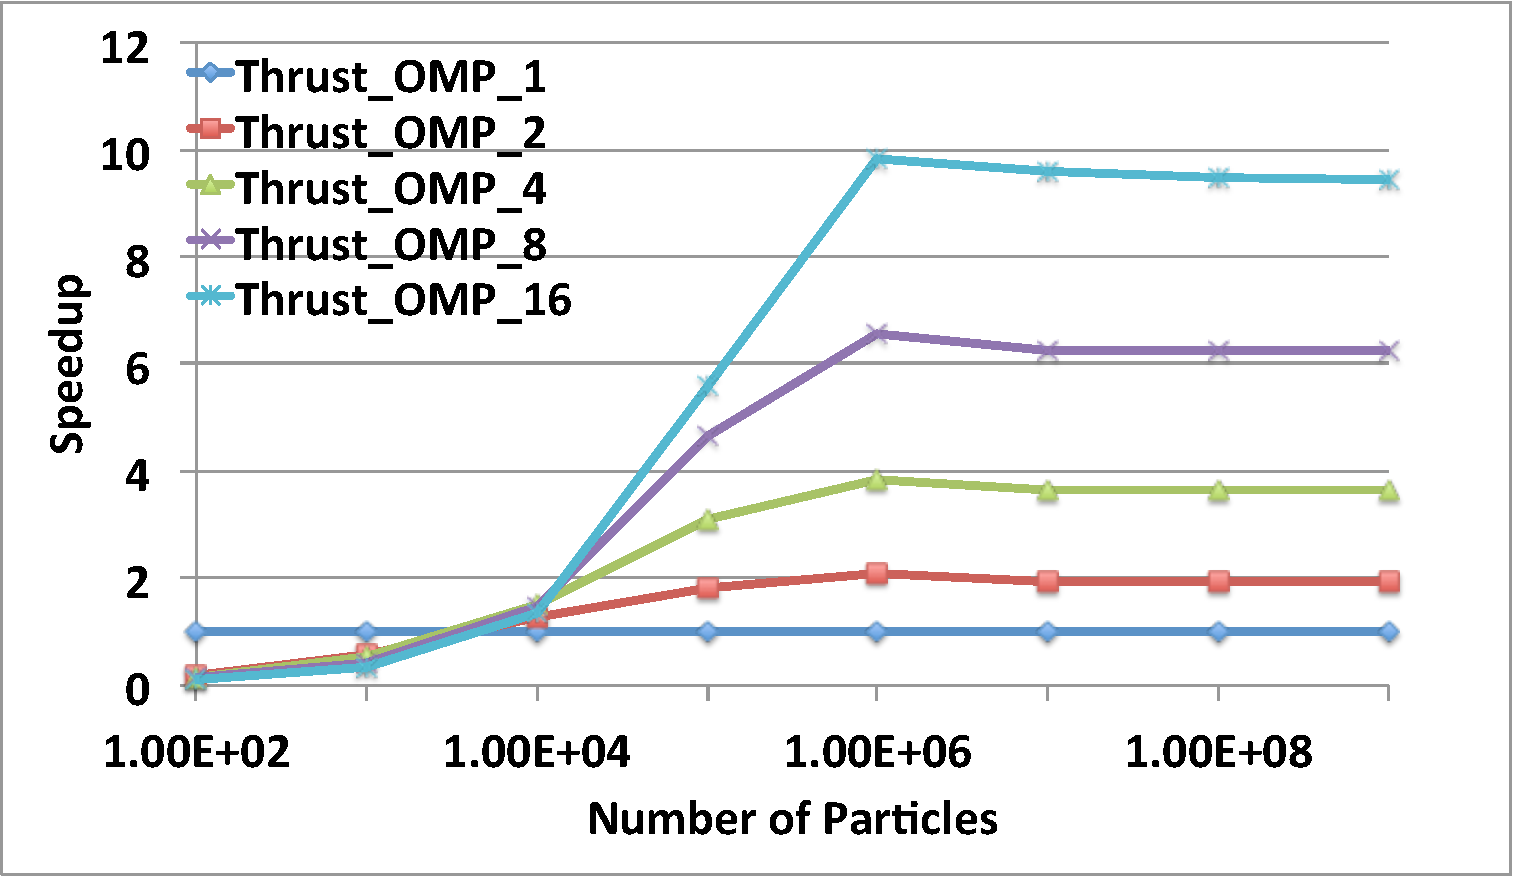
\includegraphics[width=0.49\textwidth]{thrustOMPSpeedup.pdf}
\caption{Speedups versus number of particles for the event based Thrust CPU method with 1, 2, 4, 8, 16 OpenMP threads compared to the Thrust CPU method serially.~\cite{alpsmc2}}
\label{fig:OMPScale}
\end{figure}

All of these considerations lay a foundation for future study.
%
ALPSMC is a small test code that functions like a mini app to a larger application.
%
Since ALPSMC does simplify many of the complex parts of the Monte Carlo transport problem the actual speedups may not accurately reflect the final performance possibilities of a more fully featured Monte Carlo transport code.
%

\subsection{\textbf{Proposal}}

This survey has outlined the long history of Monte Carlo transport applications and research.
%
In this survey we have seen that there has been a major revival of computational studies with every new generation of supercomputing platform.
%
Monte Carlo transport applications have only one significant gap in knowledge were groups have just recently started adding supporting research.
%
That area is the case of a fully features Monte Carlo application on GPUs and scalable to high numbers of GPUs as we will see on the next generation of supercomputers.

Previous thesis work lays a starting foundation to build upon, but does not begin to provide a full solution for other groups to follow.
%
One significant hurdle in the Monte Carlo transport world is the necessary redesign for GPU hardware.
%
It is important for groups to not need to rewrite their entire applications, which can consist of hundreds of thousands of lines of code.
%
Codes like MCNP~\cite{goorley2012initial}~\cite{padovani2012mcnpx}, Mercury~\cite{brantley2013recent}, and even OpenMC~\cite{romano2015openmc}
will all be faced with many decisions on how to progress into the future of computing.

The OpenMC group has started looking into this problem through the use of mini applications, RSBench~\cite{tramm2014performance} and XSBench~\cite{tramm2014xsbench}. 
%
This approach allows groups to focus on the specific areas that are important to them and optimize an easier to manipulate application before attempting any changes on a full scale production application.
%
One of the major focuses of this work has been in the area of continuous energy cross section searches, since for a large number of their problems that functionality took \textasciitilde85\% of their workload.

As with many other groups the Mercury group at LLNL has also begun work on a mini application.
%
This application is different to RSBench and XSBench in multiple ways but most significantly it uses the multi group energy cross sections and emphasizes  many of the key areas of the Mercy production application.
%
This application will provide a begining point for redesign of the Mercury Monte Carlo code and allow for a rich research environment for the upcomming years.
%

I propose to work under the Mercury group on the Quicksilver mini application, in order to develop a scalable GPU version of the code in a way that can translate to direct modifications of the production application.
%
I will further explore the event versus history based dilemma under the Quicksilver application in order to understand the potential performance when compared to the much larger necissary redesign.
%
I also plan on exploring the potential for a hybrid event/history algorithm that might utilize the advantages of both when possible.
%
I also plan on using the data parallel primitive design scheme as well as some layer of abstraction to make my research portable to multiple architecture platforms.
%
Additionally, there are a number of optimizations, data structures, and smaller research problems to tackle along the path of development.
%
Finally, I plan on summarizing the results of my research through large scale testing on the Trinity MIC platform, as well as the not yet released Sierra NVIDIA Volta platform.

The goal of this research will be to provide a concrete path forward for the Mercury team as well as provide a mini application that scales well on both of the competing top architectures at once.
%
This path involved many as of yet unanswered questions and a clear path of research for providing new an unique research to this field.






\nocite{*}

% references section


\bibliographystyle{IEEEtran}
\bibliography{IEEEabrv,OralsBib}


% that's all folks
\end{document}



% An example of a floating figure using the graphicx package.
% Note that \label must occur AFTER (or within) \caption.
% For figures, \caption should occur after the \includegraphics.
% Note that IEEEtran v1.7 and later has special internal code that
% is designed to preserve the operation of \label within \caption
% even when the captionsoff option is in effect. However, because
% of issues like this, it may be the safest practice to put all your
% \label just after \caption rather than within \caption{}.
%
% Reminder: the "draftcls" or "draftclsnofoot", not "draft", class
% option should be used if it is desired that the figures are to be
% displayed while in draft mode.
%
%\begin{figure}[!t]
%\centering
%\includegraphics[width=2.5in]{myfigure}
% where an .eps filename suffix will be assumed under latex, 
% and a .pdf suffix will be assumed for pdflatex; or what has been declared
% via \DeclareGraphicsExtensions.
%\caption{Simulation results for the network.}
%\label{fig_sim}
%\end{figure}

% Note that the IEEE typically puts floats only at the top, even when this
% results in a large percentage of a column being occupied by floats.


% An example of a double column floating figure using two subfigures.
% (The subfig.sty package must be loaded for this to work.)
% The subfigure \label commands are set within each subfloat command,
% and the \label for the overall figure must come after \caption.
% \hfil is used as a separator to get equal spacing.
% Watch out that the combined width of all the subfigures on a 
% line do not exceed the text width or a line break will occur.
%
%\begin{figure*}[!t]
%\centering
%\subfloat[Case I]{\includegraphics[width=2.5in]{box}%
%\label{fig_first_case}}
%\hfil
%\subfloat[Case II]{\includegraphics[width=2.5in]{box}%
%\label{fig_second_case}}
%\caption{Simulation results for the network.}
%\label{fig_sim}
%\end{figure*}
%
% Note that often IEEE papers with subfigures do not employ subfigure
% captions (using the optional argument to \subfloat[]), but instead will
% reference/describe all of them (a), (b), etc., within the main caption.
% Be aware that for subfig.sty to generate the (a), (b), etc., subfigure
% labels, the optional argument to \subfloat must be present. If a
% subcaption is not desired, just leave its contents blank,
% e.g., \subfloat[].


% An example of a floating table. Note that, for IEEE style tables, the
% \caption command should come BEFORE the table and, given that table
% captions serve much like titles, are usually capitalized except for words
% such as a, an, and, as, at, but, by, for, in, nor, of, on, or, the, to
% and up, which are usually not capitalized unless they are the first or
% last word of the caption. Table text will default to \footnotesize as
% the IEEE normally uses this smaller font for tables.
% The \label must come after \caption as always.
%
%\begin{table}[!t]
%% increase table row spacing, adjust to taste
%\renewcommand{\arraystretch}{1.3}
% if using array.sty, it might be a good idea to tweak the value of
% \extrarowheight as needed to properly center the text within the cells
%\caption{An Example of a Table}
%\label{table_example}
%\centering
%% Some packages, such as MDW tools, offer better commands for making tables
%% than the plain LaTeX2e tabular which is used here.
%\begin{tabular}{|c||c|}
%\hline
%One & Two\\
%\hline
%Three & Four\\
%\hline
%\end{tabular}
%\end{table}


% Note that the IEEE does not put floats in the very first column
% - or typically anywhere on the first page for that matter. Also,
% in-text middle ("here") positioning is typically not used, but it
% is allowed and encouraged for Computer Society conferences (but
% not Computer Society journals). Most IEEE journals/conferences use
% top floats exclusively. 
% Note that, LaTeX2e, unlike IEEE journals/conferences, places
% footnotes above bottom floats. This can be corrected via the
% \fnbelowfloat command of the stfloats package.

